\documentclass{amsart}[12pt]

\usepackage[cmtip,all]{xy}
\usepackage[utf8]{inputenc}
\usepackage{amsmath}
\usepackage{mathrsfs}
\usepackage{amssymb}
\usepackage{mathtools}
\usepackage{url}
\usepackage[top=1.3in, bottom=1.3in, left=1.3in, right=1.3in]{geometry}
\usepackage{pxfonts}
\usepackage{tikz-cd}
\usetikzlibrary{matrix,arrows}
\usepackage{hyperref}
\usepackage[boxsize=2em]{ytableau}
\usepackage{ytableau,varwidth}
\usetikzlibrary{calc}
\usepackage{eepic}
\usepackage{mathbbol}
\ytableausetup{centertableaux}
\usepackage{color}


\newtheorem{theorem}{Theorem}[section]
\newtheorem{lemma}[theorem]{Lemma}
\newtheorem{cor}[theorem]{Corollary}
\newtheorem{prop}[theorem]{Proposition}
\theoremstyle{definition}
\newtheorem{defn}[theorem]{Definition}
\newtheorem{eg}[theorem]{Example}
\newtheorem{ex}[theorem]{Exercise}
\newtheorem{fact}[theorem]{Fact}
\newtheorem{ob}[theorem]{Observation}
\newtheorem{claim}[theorem]{Claim}
\newtheorem{question}[theorem]{Question}
\newtheorem{obs}[theorem]{Observation}

\linespread{1.5}

\theoremstyle{remark}
\newtheorem{rmk}[theorem]{Remark}

\numberwithin{equation}{section}

%    Absolute value notation
\newcommand{\abs}[1]{\lvert#1\rvert}
\newcommand{\To}{\longrightarrow}
\newcommand*{\sheafhom}{\mathscr{H}\kern -.5pt om}

\begin{document}

\title{Hilbert schemes of points on surfaces with Kleinian singularities}

\author{%Xudong Zheng%\thanks{Department of Mathematics, Johns Hopkins University. \href{mailto:xzheng27@jhu.edu}{xzheng27@jhu.edu}}}      %   \and
         %etc.
}

\maketitle

\begin{abstract}
We prove that the Hilbert scheme of points on a normal quasi-projective surface with at worst Kleinian singularities is irreducible. 
%\keywords{Hilbert schemes \and maximal Cohen-Macaulay modules \and Kleinian singularities}
\end{abstract}

\section{Introduction}

Let $X$ be an integral quasi-projective surface over the field of complex numbers with Kleinian singularities. In this paper, we prove that the Hilbert scheme $\mathrm{Hilb}^d(X)$ of $d$ points on $X$ is irreducible for any integer $d$. It is well-known that the Hilbert scheme $\mathrm{Hilb}^d(X)$ on a non-singular surface $X$ is non-singular and connected, in particular, irreducible (\cite[Proposition 2.3, Theorem 2.4]{F68}), whereas $\mathrm{Hilb}^d(X)$ is reducible for sufficiently large $d$ if $X$ has an isolated cone singularity over a non-singular curve of degree at least $5$ (\cite[Theorem 2.5]{MP13}). 

Kleinian singularities (du Val singularities, simple surface singularities, rational double points) are the 2-dimensional canonical singularities. Kleinian singularities are quotient singularities. For each Kleinian singularity, there are finitely many isomorphism classes of indecomposable reflexive modules (\cite{H78}, also see \cite[Proposition 2.1]{A86}), and their Auslander-Reiten sequences are well-understood via the McKay correspondence (\cite[Proposition 2.1, 3.2]{A86}). The goal of this paper is to investigate the irreducibility of Hilbert schemes of points on surfaces with Kleinian singularities. The main result is the following

\begin{theorem}\label{theorema}
Let $X$ be a quasi-projective normal surface with at worst Kleinian singularities, and let $d$ be a positive integer. Denote by $\mathrm{Hilb}^d(X)$ the Hilbert scheme of length $d$ subschemes of $X$. Then $\mathrm{Hilb}^d(X)$ is irreducible of dimension $2d$ for any $d$.
\end{theorem}

The strategy of the proof of Theorem \ref{theorema} is as follows.
\begin{itemize}
\item[(i)] The Hilbert scheme $\mathrm{Hilb}^d(X)$ is irreducible if and only if any length $d$ subscheme of $X$ is \textit{smoothable}, i.e., a flat specialization of $d$ distinct points. It suffices that any length $d$ subscheme of $X$ supported at a single singular point is smoothable, and it suffices to assume that $X$ is the spectrum of an analytic germ of a Kleinian singularity. 
\item[(ii)] A deformation of the first syzygy module of a length $d$ subscheme of the surface singularity induces a flat embedded deformation of the subscheme (Proposition \ref{families}).
\item[(iii)] A subscheme of finite projective dimension is smoothable (Proposition \ref{finitehd}).
\item[(iv)] The first syzygy module of any length $d$ subscheme is the specialization of free modules of the same rank (Proposition \ref{key}). 
\end{itemize}

Furthermore, if we reduce to the affine case with $X = \mathbb{C}^2/\Gamma$ the quotient of $\mathbb{C}^2$ by a finite group $\Gamma \leq \mathrm{SL}(2, \mathbb{C})$, an explicit resolution of singularities of $\mathrm{Hilb}^d(X)$ can be constructed. This smooth birational model as a resolution of singularities of the $d$-th symmetric product $X^{(d)}$ after composing with the Hilbert-Chow morphism $h: \mathrm{Hilb}^d(X) \to X^{(d)}$ carries a holomorphic symplectic 2-form extended from the regular locus of $X^{(d)}$. In particular, $\mathrm{Hilb}^d(X)$ admits a symplectic resolution. The study of this resolution and related questions will appear in a sequel of this article. 

The paper is organized as follows. In section 2, we review the McKay correspondence for Kleinian singularities and the construction of some short exact sequences of reflexive modules over Kleinian singularities. Section 3 contains the technical results on the deformations of reflexive modules in the context of Kleinian singularities. In section 4, we prove Theorem \ref{theorema} through a case-by-case analysis according to the singularity types. The converse of Theorem \ref{theorema} is partially supported by Example \ref{cevv}. Auslander-Reiten theory and ladders in $\tau$-categories are recalled in the Appendix.



\section{Preliminaries}
Let $X$ be a quasi-projective surface over $\mathbb{C}$. For any positive integer $d$, the Hilbert scheme of $d$ points, denoted by $\mathrm{Hilb}^d(X)$, is the moduli space of zero-dimensional subschemes of $X$ of length $d$. 

A \textit{surface singularity} $(X, p)$ refers to the spectrum of a two-dimensional analytic germ. The singularity $(X, p)$ is said to be \textit{rational} if the higher direct image sheaf $\mathbf{R}^i\pi_*\mathcal{O}_Y$ is zero for $i > 0$ and for any resolution $\pi: Y \to (X, p)$ of the singularity.

\begin{prop}\label{smoothness}
Suppose $X$ is a quasi-projective surface with only isolated rational singularities, and $Z$ is a zero-dimensional subscheme of $X$ of length $d$. If $Z$ has finite projective dimension on $X$, then the dimension of the Zariski tangent space of $\mathrm{Hilb}^d(X)$ at $[Z]$ is $2d$.
\begin{proof}
The Zariski tangent space of $\mathrm{Hilb}^d(X)$ at $[Z]$ is isomorphic to $\mathrm{Hom}_{\mathcal{O}_X}(\mathcal{I}_Z, \mathcal{O}_Z)$. By assumption, any projective resolution of the ideal sheaf $\mathcal{I}_Z$ of $Z$ on $X$ is finite. The Auslander-Buchsbaum formula implies that such a resolution has length 1. By the theorem of Hilbert-Burch-Schaps, an $\mathcal{O}_X$-free resolution of $\mathcal{I}_Z$ has the form:
\begin{equation}\label{ses}
0 \to \mathcal{O}_X^{\oplus r} \to \mathcal{O}_X^{\oplus r + 1} \to \mathcal{I}_Z \to 0.
\end{equation}
Applying $\mathrm{Hom}(\bullet, \mathcal{O}_Z)$ to (\ref{ses}), it follows that $\mathrm{Ext}^j(\mathcal{I}_Z, \mathcal{O}_Z) = 0$ for any $j \geq 2$, and that the following sequence is exact:
\begin{equation}\label{fourterm}
0 \to \mathrm{Hom}(\mathcal{I}_Z, \mathcal{O}_Z) \to \mathrm{Hom}( \mathcal{O}_X^{\oplus r}, \mathcal{O}_Z) \to \mathrm{Hom}( \mathcal{O}_X^{\oplus r + 1}, \mathcal{O}_Z) \to  \mathrm{Ext}^1(\mathcal{I}_Z, \mathcal{O}_Z) \to 0.
\end{equation}
Applying $\mathrm{Hom}(\bullet, \mathcal{O}_Z)$ to $0 \to \mathcal{I}_Z \to \mathcal{O}_X \to \mathcal{O}_Z \to 0$ and by duality, it follows that $\mathrm{Ext}^1(\mathcal{I}_Z, \mathcal{O}_Z) \cong \mathrm{Ext}^2(\mathcal{O}_Z, \mathcal{O}_Z) \cong \omega_Z$, and $\dim_{\mathbb{C}} \mathrm{Ext}^1(\mathcal{I}_Z, \mathcal{O}_Z) = d$. Counting dimensions on the terms of the sequence (\ref{fourterm}) we see that $\dim_{\mathbb{C}} \mathrm{Hom}(\mathcal{I}_Z, \mathcal{O}_Z) = 2d$.
\end{proof}
\end{prop}

\begin{rmk}
In fact, under the assumptions of Proposition \ref{smoothness} $\mathrm{Hilb}^d(X)$ is smooth at $[Z]$. Consider the exact sequence 
\[
H^1(Z, \mathcal{H}om_Z(I_Z, \mathcal{O}_Z)) \hookrightarrow \mathrm{Ext}^1_Z(I_Z, \mathcal{O}_Z) \xrightarrow{rest} H^0(Z, \mathcal{E}xt^1_Z(I_Z, \mathcal{O}_Z))
\]
The map $rest$ is the restriction from the global to local obstructions (cf. the proof of \cite[Claim I. 2.14.5]{K96}). Since $Z$ has  projective dimension 1, $Z$ is determinantal. There is infinitesimal lifting of the matrix defining $Z$, hence there is no local obstruction to a flat deformation of $Z$ (see \cite[Theorem 5.1]{A76}). Notice that $\mathcal{H}om_Z(I_Z, \mathcal{O}_Z)$ is supported on $Z$, hence $H^1(Z, \mathcal{H}om_Z(I_Z, \mathcal{O}_Z)) = 0$. Therefore, $\mathrm{Ext}^1_Z(I_Z, \mathcal{O}_Z) = 0$. 
\end{rmk}

Suppose $(B, \mathfrak{m})$ is a Noetherian local ring, and $M$ is a finitely generated $B$-module. Then $M$ is \textit{maximal Cohen-Macaulay}, or \textit{MCM}, if $M$ satisfies $\mathrm{depth}(M) = \dim B$; $M$ is \textit{reflexive}, if $M \cong M^{**}$, where $(\bullet)^* = \mathrm{Hom}_B(\bullet, B)$. If $(X, p)$ is a surface singularity, then MCM $\mathcal{O}_{X, p}$-modules are precisely the reflexive $\mathcal{O}_{X, p}$-modules. If $Z$ is any zero-dimensional subscheme of $X$ supported at $p$, then its first syzygy module $\mathcal{M}_Z$ is a reflexive $\mathcal{O}_{X, p}$-module.
 
\begin{prop}\label{families}
Let $X$ be a quasi-projective surface with only rational singularity, and $Z$ be a zero-dimensional subscheme of $X$ of length $d$. Denote the first syzygy module of $Z$ by $\mathcal{M}_Z$. Suppose $\mathcal{M}_Z$ has rank $r$. Suppose $\{\mathcal{M}_t\}$ is a connected flat 1-parameter family of reflexive $\mathcal{O}_X$-modules over $\mathbb{A}^1$ such that $\mathcal{M}_0 \cong \mathcal{M}_Z$ and $\mathcal{M}_t$ is a submodule of $\mathcal{O}_X^{\oplus r + 1}$ for any $t \in \mathbb{A}^1$. Then there exist length $d$ subschemes $Z_t$ of $X$ for each $t$ in some open neighborhood $\emptyset \neq V \subset \mathbb{A}^1$ of 0 such that $\mathcal{M}_t$ is isomorphic to the first syzygy module of $Z_t$ for any $t \in V$.
\begin{proof}
Denote by $\mathfrak{X} = X \times \mathbb{A}^1$ the isotrivial 1-parameter family of surfaces with two projections $\pi_X: \mathfrak{X} \to X$ and $\pi_{\mathbb{A}^1}: \mathfrak{X} \to \mathbb{A}^1$. By assumption, there are exact sequences $0 \to \mathcal{M}_0 \xrightarrow{\phi_0} \mathcal{O}_X^{\oplus r + 1} \to \mathcal{I}_Z \to 0$ and $0 \to \mathcal{F}_1 \xrightarrow{\phi} \mathcal{F}_0$, which satisfy the following properties:
\begin{itemize}
\item[(i)] $\mathcal{F}_1$ and $\mathcal{F}_0$ are $\mathcal{O}_{\mathfrak{X}}$-modules such that the restriction of $\phi$ to the closed fiber $X_0 \cong X$ over $0 \in \mathbb{A}^1$ is $\phi_0$;
\item[(ii)] $\mathcal{F}_0$ is a free $\mathcal{O}_{\mathfrak{X}}$-module of rank $r + 1$;
\item[(iii)] $\mathcal{F}_1$ is a reflexive $\mathcal{O}_{\mathfrak{X}}$-module of rank $r$ with $\mathrm{depth}_q(\mathcal{F}_1) = 3$ for any closed point $q \in \mathfrak{X}$.
\end{itemize}

Let $\mathcal{Q}$ be the cokernel sheaf of $\phi$. Then $\mathcal{Q} \vert_{X_0} \cong \mathcal{I}_Z$. To construct the desired family of zero-dimensional subschemes of $X$, it suffices to show that the restriction of $\mathcal{Q}$ to an open neighborhood of $0$ in $\mathbb{A}^1$ is a flat family of ideal sheaves of length $d$ subschemes. 

The support of the torsion part $\mathcal{Q}_{tor}$ of $\mathcal{Q}$, if non-empty, is disjoint from the closed fiber $X_0$ by property (i). Denote by $U_1 \subset  \mathbb{A}^1$ the complement of $\pi_{\mathbb{A}^1}(\mathrm{Supp} (\mathcal{Q}_{tor}))$, by $\mathfrak{X}_1 = X \times U_1$ the restricted family, and by $\mathcal{Q}_1$ the restriction of $\mathcal{Q}$ to $\mathfrak{X}_1$. Then $\mathcal{Q}_1$ is a rank 1 torsion free sheaf on $\mathfrak{X}_1$ such that $\mathcal{Q}_1 \vert_{X_0} \cong \mathcal{I}_Z$. The double dual $\mathcal{Q}_1^{**}$ of $\mathcal{Q}_1$ is a rank 1 reflexive $\mathcal{O}_{\mathfrak{X}_1}$-module. Then there exists a Weil divisor $D$ of $\mathfrak{X}_1$ such that $\mathcal{Q}_1^{**} \cong \mathcal{O}_{\mathfrak{X}_1}(D)$. 

The restriction map of divisor class groups $p: \mathrm{Cl}(\mathfrak{X}) \to \mathrm{Cl}(\mathfrak{X}_1)$ is surjective, and $\mathrm{Cl}(\mathfrak{X})$ is isomorphic to $\mathrm{Cl}(X)$ since $\mathfrak{X}$ is an isotrivial family of $X$ over $\mathbb{A}^1$. Hence there exists a Weil divisor $D_0$ of $X$ such that $p^* \mathcal{O}_{\mathfrak{X}_1}(D) \cong \pi_X^*\mathcal{O}_{X}(D_0)$. Restricting this isomorphism to $X_0$ it follows that $D_0$ is homologous to 0, so it is with $D$. Therefore, $\mathcal{Q}_1^{**} \cong \mathcal{O}_{\mathfrak{X}_1}$. Then there is a closed subscheme $W$ of $\mathfrak{X}_1$ such that $\mathcal{Q}_1 \cong \mathcal{I}_W$. In particular, $W \vert_{X_0} \cong Z$.

If $W$ is flat over $U_1$ then we are done. Otherwise, there are two possibilities: (1) $W$ is not equi-dimensional and it contains 2-dimensional components, and (2) $W$ is purely 1-dimensional and some components are contracted by $\pi_{\mathbb{A}^1}$. Denote by $W_1$ the union of the 2-dimensional components of $W$. By the condition $W \vert_{X_0} \cong Z$ again, $W_1$ is disjoint from $X_0$. Denote by $\mathfrak{X}_2 = \mathfrak{X}_1 \setminus W_1$ the complement of $W_1$, which is non-empty open in $\mathfrak{X}$. It follows that $\mathcal{Q}_1 \vert_{\mathfrak{X}_2}$ is isomorphic to the ideal sheaf of a 1-dimensional scheme $W_2$. By property (iii) on the depth of $F_1$, the scheme $W_2$ is a Cohen-Macaulay curve. If $C$ is any component of $W_2$ that is contracted by $\pi_{\mathbb{A}^1}$, then $\pi_{\mathbb{A}^1}(C) \neq 0$. Hence there exists an open neighborhood $U_2$ of $0$ such that $W_2$ is flat over $U_2$. In particular, each fiber of $W_2$ over $U_2$ is a finite subscheme of $X$ of the same length as $Z$.
\end{proof}
\end{prop}

A surface singularity $(X, p)$ is \textit{Kleinian} if $(X, p)$ admits a resolution of singularity such that the dual graph is one of the types $A_n, D_n, E_6, E_7$, or $E_8$. Kleinian singularities are the analytic germs of quotients of $\mathbb{A}^2$ by a finite subgroup $\Gamma \leq \mathrm{SL}(2, \mathbb{C})$. The action of $\Gamma \leq \mathrm{SL}(2, \mathbb{C})$ on $S = \mathbb{C}\llbracket x, y\rrbracket$ is induced by the action of $\mathrm{SL}(2, \mathbb{C})$. Denote bt $R \cong S^{\Gamma}$ the ring of $\Gamma$-invariants. 

From now on, $(X, p)$ will always denote a Kleinian singularity, and $X = \mathrm{Spec}(R)$.

The \textit{McKay correspondence} is the bijection of the following three finite sets:
\begin{align*}
\mathcal{M}_1 & = \{\textrm{non-trivial isomorphism classes of irreducible representations of $\Gamma$}\} \\
\mathcal{M}_2 & = \{\textrm{non-trivial isomorphism classes of indecomposable reflexive modules over $R$}\} \\
\mathcal{M}_3 & = \{\textrm{irreducible components of the exceptional divisor in the minimal resolution of $(X, p)$}\}
\end{align*}

The correspondence between $\mathcal{M}_1$ and $\mathcal{M}_2$ plays a key role in this article. The \textit{skew group ring} $S[\Gamma]$ of $\Gamma$ over $S$ is the free $S$-module over the basis of elements of $\Gamma$, whose multiplication is defined so that $(s_1g_1)(s_2g_2) = s_1g_1(s_2)g_1g_2$ for any $s_1, s_2 \in S$ and $g_1, g_2 \in \Gamma$. Then an $S[\Gamma]$-module $M$ is an $S$-module with a $\Gamma$-action: $g(sm) = g(s)g(m)$ for any $g \in \Gamma, s \in S$, and $m \in M$. Any indecomposable projective $S[\Gamma]$-module up to isomorphism corresponds to an irreducible representation of $\Gamma$ up to isomorphism and vice versa.

\begin{prop}\cite[Lemma 1.1, Proposition 2.1, Proposition 2.2]{A86}\label{equicat}
\begin{itemize}
\item[(i)] An $S[\Gamma]$-module is projective if and only if it is a free $S$-module. 
\item[(ii)] There is an equivalence between the following three categories: the category $\mathfrak{P}$ of projective $S[\Gamma]$-modules, the category $MCM(R)$ of reflexive $R$-modules, and the category $\mathrm{add}(S)$ of $S$-modules that are submodules of some free $S$-modules. 
\end{itemize}
\end{prop}

By Proposition \ref{equicat}, the correspondence between $\mathcal{M}_1$ and $\mathcal{M}_2$ is the restriction of the equivalence $\mathfrak{P} \cong MCM(R)$. Let $\rho_1, \dots, \rho_n$ be the isomorphism classes of non-trivial irreducible representation of $\Gamma$, $P_1, \dots, P_n$ be the isomorphism classes of indecomposable projective $S[\Gamma]$-modules, and $M_1, \dots, M_n$  be the isomorphism classes of indecomposable reflexive $R$-modules. Then $\rho_i \otimes_{\mathbb{C}} S \cong P_i$ and $P_i^{\Gamma} \cong M_i$ for $i = 1, \dots, n$. By \cite[Lemma 3.1(a)]{A86}, the correspondence $\mathcal{M}_1 \to \mathcal{M}_2$ preserves taking dual. For the correspondence between $\mathcal{M}_3$ and $\mathcal{M}_2$, see \cite{AV85}.

Let $\rho$ be the natural 2-dimensional representation of $\Gamma$. The \textit{affine Dynkin diagram} is a finite graph with $n + 1$ vertices corresponding to the representations $\rho_0 \cong \mathbb{C}, \rho_1, \dots, \rho_n$ such that there is an edge between the vertex $i$ and vertex $j$ if $\rho_i$ is a summand of $\rho_j \otimes \rho$. (If so, then $\rho_j$ is also a summand of $\rho_i \otimes \rho$.) For an indecomposable reflexive $R$-module $M_i$, denote by $E(M_i)$ the reflexive $R$-module corresponding to $\rho_i \otimes \rho$, then $E(M_i)$ is the direct sum of modules $M_j$ over all indices $j$ connected to $i$ by an edge in the affine Dynkin diagram. By \cite[Proposition 3.2]{A86}, there is an exact sequence of reflexive $R$-modules $0 \to M_i \to E(M_i) \xrightarrow{\alpha} M_i \to 0$, which satisfies the following properties for $i = 1, \dots, n$. 
\begin{itemize}
\item[(i)] The sequence does not split.
\item[(ii)] Every morphism $h: M \to M_i$ of reflexive $R$-modules which is not a splittable epimorphism can be lifted to $E(M_i)$, i.e., there is a morphism $\beta: M \to E(M_i)$ such that $h = \alpha \circ \beta$.
\end{itemize}

This sequence is called the \textit{Auslander-Reiten sequence} of $M_i$ (in \cite{A86}, it is called the \textit{almost split sequence} determined by $M_i$). The Auslander-Reiten sequence of $M_i$ is uniquely determined by $M_i$ for each $M_i$. 

By \cite[Corollary 1.3]{HK}, the minimal number of generators of any non-trivial indecomposable reflexive $R$-module $M_i$ is $2 \mathrm{rk}\, M_i$. By \cite[Theorem 6.1(ii)]{E80}, any non-trivial indecomposable reflexive $R$-module $M_i$ admits a 2-periodic $R$-free resolution. For any $R$-module $M$, we denote by $\mathrm{Syz}_1(M)$ the kernel of a surjection $R^{\oplus n} \to M$ for minimal possible $n$, and it is referred as the \textit{syzygy module} of $M$. In particular, If $M_i$ is reflexive, then $\mathrm{Syz}_1(M_i)$ is reflexive and $\mathrm{rk}\, M_i = \mathrm{rk}\, \mathrm{Syz}_1(M_i)$.

Denote by $\hat{\Gamma}$ the character group of $\Gamma$. Then $\hat{\Gamma} \cong \mathrm{Cl}(R)$, the divisor class group of $R$. Explicitly, 
\[
\hat{\Gamma} \cong \begin{cases}
\mathbb{Z}/(n + 1)\mathbb{Z} & A_n \\
\mathbb{Z}/(2) \oplus \mathbb{Z}/(2) & D_{2k} \\
\mathbb{Z}/(4) & D_{2k + 1} \\
\mathbb{Z}/(3) & E_6 \\
\mathbb{Z}/(2) & E_7 \\
\{1\} & E_8
\end{cases}
\]

Since $R$ is normal, any reflexive $R$-module $M$ gives rise to a class in $\mathrm{Cl}(R)$ by taking determinant of $M$, and is denoted by $[M]$. 

\begin{center}
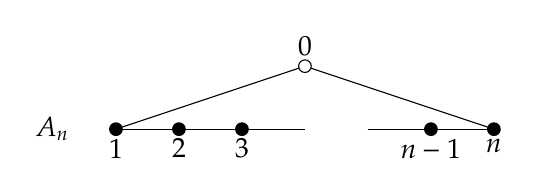
\begin{tikzpicture}[scale = .8]
\draw (0,0) -- (3,1);
\draw (6,0) -- (3,1);
\draw (0,0) -- (3,0);
\draw (4,0) -- (6,0);
\draw[fill=black] (0,0)                     
      circle [radius=.1] node [below] {1} ;
     \draw[fill=black]  (1,0)                       
      circle [radius=.1] node [below] {2};
     \draw[fill=black]  (2,0)                         
      circle [radius=.1] node [below] {3} ; 
     \draw[fill=black]  (5,0)                         
      circle [radius=.1] node [below] {$n - 1$};
     \draw[fill=black]  (6,0)                         
      circle [radius=.1] node [below] {$n$};
      \draw[fill=white] (3,1) circle(.1) node [above] {0};
      
      \node at (-1,0) {$A_n$};
\end{tikzpicture}
\end{center}

\begin{center}
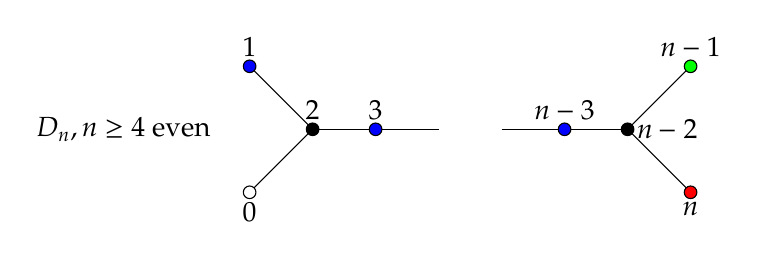
\begin{tikzpicture}[scale = .8]
\draw (0,1) -- (1,0);
\draw (0,-1) -- (1,0);
\draw (1,0) -- (3,0);
\draw (4,0) -- (6,0);
\draw (6,0) -- (7, 1);
\draw (6,0) -- (7, -1);
\draw[fill=blue] (0,1)                         
      circle [radius=.1] node [above] {1};
     \draw[fill=black]  (1,0)                         
      circle [radius=.1] node [above] {2};
     \draw[fill=blue]  (2,0)                         
      circle [radius=.1] node [above] {3}; 
     \draw[fill=blue]  (5,0)                         
      circle [radius=.1] node [above] {$n - 3$};
\draw[fill=black] (6,0) 
      circle [radius=.1] node [right] {$n - 2$}; 
     \draw[fill=green]  
(7, 1)
      circle [radius=.1] node [above] {$n - 1$};
      \draw[fill=red]
(7, -1)
      circle [radius=.1] node [below] {$n$}      
      ;
      \draw[fill=white] (0,-1) circle(.1) node [below] {0};
      \node at (-2,0) {$D_n, n \geq 4$ even};
\end{tikzpicture}
\end{center}

\begin{center}
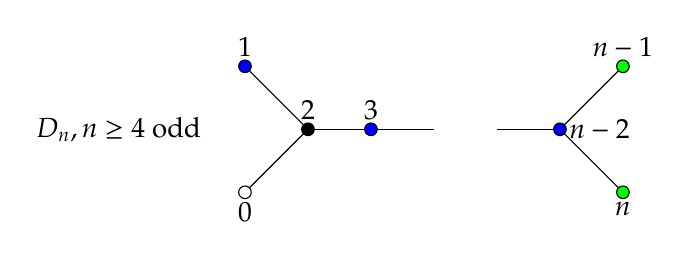
\begin{tikzpicture}[scale = .8]
\draw (0,1) -- (1,0);
\draw (0,-1) -- (1,0);
\draw (1,0) -- (3,0);
\draw (4,0) -- (5,0);
\draw (5,0) -- (6, 1);
\draw (5,0) -- (6, -1);
\draw[fill=blue] (0,1)                         
      circle [radius=.1] node [above] {1};
     \draw[fill=black]  (1,0)                         
      circle [radius=.1] node [above] {2};
     \draw[fill=blue]  (2,0)                         
      circle [radius=.1] node [above] {3}; 
\draw[fill=blue] (5,0) 
      circle [radius=.1] node [right] {$n - 2$}; 
     \draw[fill=green]  
(6, 1)
      circle [radius=.1] node [above] {$n - 1$};
      \draw[fill=green]
(6, -1)
      circle [radius=.1] node [below] {$n$}      
      ;
      \draw[fill=white] (0,-1) circle(.1) node [below] {0};
      \node at (-2,0) {$D_n, n \geq 4$ odd};
\end{tikzpicture}
\end{center}

\begin{center}
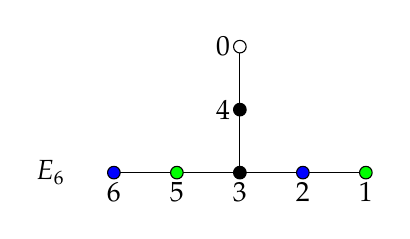
\begin{tikzpicture}[scale = .8]

	\draw (0,0) -- (4,0);
	\draw (2,0) -- (2,1);
	\draw (2,2) -- (2,1);
	
	\draw[fill=blue] (0,0) circle(.1) node [below] {6};
	\draw[fill=green] (1,0) circle(.1) node [below] {5};
	\draw[fill=black] (2,0) circle(.1) node [below] {3};
	\draw[fill=black] (2,1) circle(.1) node [left] {4};
	
	\draw[fill=white] (2,2) circle(.1) node [left] {0};
	\draw[fill=blue] (3,0) circle(.1) node [below] {2};
	\draw[fill=green] (4,0) circle(.1) node [below] {1};
	
	\node at (-1,0) {$E_6$};
	 
\end{tikzpicture}
\end{center}

\begin{center}
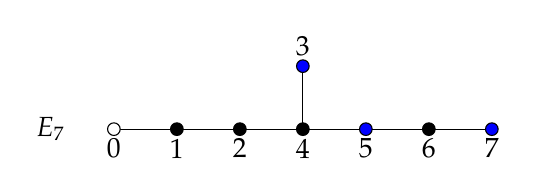
\begin{tikzpicture}[scale = .8]

	\draw (0,0) -- (5,0);
	\draw (2,0) -- (2,1);
	\draw (0,0) -- (-1,0);
	
	\draw[fill=black] (0,0) circle(.1) node [below] {1};
	\draw[fill=black] (1,0) circle(.1) node [below] {2};
	\draw[fill=black] (2,0) circle(.1) node [below] {4};
	\draw[fill=blue] (2,1) circle(.1) node [above] {3};
	\draw[fill=blue] (3,0) circle(.1) node [below] {5};
	\draw[fill=black] (4,0) circle(.1) node [below] {6};
	\draw[fill=blue] (5,0) circle(.1) node [below] {7};
	\draw[fill=white] (-1,0) circle(.1) node [below] {0};

	\node at (-2,0) {$E_7$};
	 
\end{tikzpicture}
\end{center}
\begin{center}
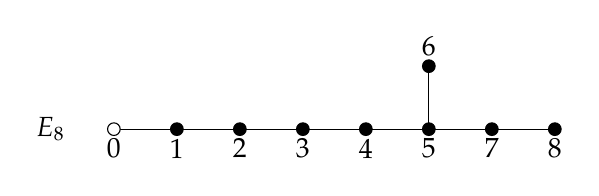
\begin{tikzpicture}[scale = .8]

	\draw (0,0) -- (6,0);
	\draw (4,0) -- (4,1);
	\draw (0,0) -- (-1,0);
	
	\draw[fill=black] (0,0) circle(.1) node [below] {1};
	\draw[fill=black] (1,0) circle(.1) node [below] {2};
	\draw[fill=black] (2,0) circle(.1) node [below] {3};
	\draw[fill=black] (3,0) circle(.1) node [below] {4};
	\draw[fill=black] (4,0) circle(.1) node [below] {5};
	\draw[fill=black] (4,1) circle(.1) node [above] {6};
	\draw[fill=black] (5,0) circle(.1) node [below] {7};
	\draw[fill=black] (6,0) circle(.1) node [below] {8};
	\draw[fill=white] (-1,0) circle(.1) node [below] {0};
	\node at (-2,0) {$E_8$};
\label{dynkin}    	 
\end{tikzpicture}


\small{Affine Dynkin diagrams of Kleinian singularities. In cases of $D_n$ and $E_n$ nodes of the same color correspond to modules with the same determinant in the divisor class group of the singularity.}
\end{center}
   % Give a unique label

For a Kleinian singularity, the module $M_i$ refers to the unique indecomposable reflexive module corresponding to the vertex indexed by $i$ for $i \neq 0$ in the preceding diagram; $M_0 \cong R$ refers to the trivial module corresponding to the vertex ``0''.

\section{Deformations of reflexive modules}
A length $d$ subscheme $Z$ of some scheme $X$ is said to be \textit{smoothable} if there exists a family $\tilde{Z}$ of length $d$ subschemes of $X$ over some Noetherian connected scheme $T$ with special fiber $Z$ and smooth general fiber.

\begin{prop}\label{finitehd}
Suppose $(X = \mathrm{Spec}(R), p)$ is a Kleinian singularity and $Z_0$ is a length $d$ subscheme of $X$ supported at $p$ with ideal $I_0$. Assume that $I_0$ has a finite free resolution on $X$. Then $Z_0$ is smoothable in $X$. 
\begin{proof}
The finiteness of the minimal $R$-free resolution of $I_0$ implies that the resolution has the form
\begin{equation}\label{fhd}
0  \to R^{\oplus r} \xrightarrow{\phi_0} R^{\oplus r + 1} \to I_0 \to 0.
\end{equation}
by the Auslander-Buchsbaum formula, where $\phi_0$ is an $(r + 1) \times r$ matrix whose entries $f_{ij}$ are non-units of $R$ such that the maximal minors give rise to the minimal set of generators of $I_0$. As in the proof of Proposition \ref{families} there is a short exact sequence (after possibly restricted to an open neighborhood of $0 \in \mathbb{A}^1$) $0  \to R[t]^{\oplus r} \xrightarrow{\phi} R[t]^{\oplus r + 1} \to \mathcal{Q} \to 0$ such that $\mathcal{Q} = \mathcal{I}_W$ is the ideal sheaf of some closed subscheme $W$ of $\mathfrak{X}$, finite and flat over an open neighborhood of $0 \in \mathbb{A}^1$.

We define a 1-parameter family of matrices: $\tilde{\phi} = \phi + tI_{r}'$, where $I_{r}' = \begin{bmatrix}
I_{r} \\
0
\end{bmatrix}$.

For $t = 0$, we have $\tilde{\phi}_0 = \phi_0$, and for any $t \neq 0$, the top $r \times r$-minor of $\tilde{\phi}$ is invertible since its determinant is $t^{r}$. Thus, $\mathrm{coker} (\tilde{\phi}_t) = I_Z$ for a closed subscheme $Z_t$ of $X$ of length $d$ such that $p \not\in \mathrm{Supp}(Z_t)$ for $t \neq 0$. 
\end{proof}
\end{prop}


\begin{lemma}\label{generic}
\begin{itemize}
\item[(i)] Let $M_j$ and $M_j$ be any non-trivial reflexive $R$-modules such that $[M_i] + [M_j] = 0 \in \mathrm{Cl}(R)$. Then there is an open dense subset of $\mathrm{Ext}^1_R(M_i, M_j)$ in which any extension is represented by $0 \to M_j \to R^{\oplus  \mathrm{rk}\, M_i + \mathrm{rk}\, M_j} \to M_i \to 0$.
\item[(ii)] Let $M_i$ and $M_j$ be any indecomposable reflexive $R$-modules. Suppose $\eta, \eta' \in \mathrm{Ext}^1_R(M_i, M_j)$ are represented by $0 \to M_j \to M \oplus R^{\oplus a} \to M_i \to 0$ and $0 \to M_j \to N \oplus R^{\oplus b} \to M_i \to 0$ respectively. Suppose $a < b$. Then $M$ can be generalized to a reflexive module with a free summand of rank at least $b$. In particular, $M \oplus \mathrm{Syz}_1(M)$ can be generalized to $R^{\oplus 2 \mathrm{rk} \, M}$ for any non-trivial indecomposable reflexive $R$-module $M$. 
\end{itemize}
\end{lemma}
\begin{proof}
(i) Any $R$-module $M$ that is represented by an extension as $0 \to M_j \to M \to M_i \to 0$ is reflexive. The minimal number of generators of $M$ is at least $\mathrm{rk}\, M = \mathrm{rk}\, M_i + \mathrm{rk}\, M_j$, and equality occurs if and only if $M$ is a free $R$-module. By upper semi-continuity of the minimal number of generators of a family of $R$-modules, there is an open dense subset of $\mathrm{Ext}^1_R(M_i, M_j)$ in which any extension represents an $R$-module with the least minimal number of generators, namely, $\mathrm{rk}\, M_i + \mathrm{rk}\, M_j$. 

(ii) Both statements follow from part (i). 
\end{proof}


An $R$-module $M$ is reflexive if and only if there exists a four-term exact sequence of $R$-modules
\[
0 \to M \to R^{\oplus a} \to R^{\oplus b} \to N \to 0
\]
where the middle terms are free $R$-modules for some $R$-module $N$ (\cite[Lemma 1.1(a)]{AR89}). We call a reflexive $R$-module $M$ a \textit{second syzygy module} if the preceding sequence can be chosen so that $N$ is a finite length module. 

\begin{prop}\label{key}
Any second syzygy module $M$ can be generalized to a free module of the same rank, namely, there is a connected flat irreducible family of reflexive modules for which the general member of the family is a free $R$-module, and the special member is the module $M$. 
\end{prop}

The determinant of any second syzygy module is trivial in $\mathrm{Cl}(R)$. Hence, for the proof of Proposition \ref{key}, it is sufficient to prove

\begin{prop}\label{keyy}
Every reflexive $R$-module whose determinant is trivial can be generalized to a free module of the same rank.
\end{prop}

The proof of Proposition \ref{keyy} is separated into 5 cases ($A_n, D_n, E_6, E_7$, and $E_8$), which involves explicit constructions of short exact sequences of reflexive modules. First, considering the depths of modules, we have

\begin{lemma}\label{injective}\cite[Part II. Lemma 1.1(c)]{AR89}
Suppose $f: M \to N$ is any morphism between reflexive $R$-modules. Then $\ker(f)$ is a reflexive $R$-module.
\end{lemma}

\begin{lemma}\label{an} Suppose $(X, p)$ is an $A_n$ singularity.
\begin{itemize}
\item[(i)] Suppose $M = R^{\oplus a} \oplus M_1^{\oplus a_1} \oplus \dots \oplus M_n^{\oplus a_{n}}$ has trivial determinant. Then $a_1 + 2a_2 + \dots + na_n$ is divisible by $n + 1$.
\item[(ii)] For any pair of indecomposable reflexive $R$-modules $M_a$ and $M_b$ for some $0 \leq a, b \leq n$, any extension of $M_b$ by $M_a$ can be represented by a short exact sequence of the form $0 \to M_a \to M_{c} \oplus M_{d} \to M_b \to 0$,
where $c + d \equiv a + b \mod n + 1$. In particular, there is the following exact sequence $0 \to M_a \to M_{a - i} \oplus M_{b + i} \to M_b \to 0$, for any $0 \leq i \leq \max\{a, n + 1 - b\}$. 
\item[(iii)] The direct sum $M_b \oplus M_a$ can be realized as the specialization of $R \oplus M_{\overline{a + b}}$, where $\overline{a + b} \equiv a + b \mod n + 1$, and $0 \leq \overline{a + b} \leq n$. 
\end{itemize}
\begin{proof}
(i) Via the isomorphism $\mathrm{Cl}(R) \cong (\mathbb{Z}/(n + 1)\mathbb{Z}, +)$, the class $[M_i]$ is identified with the congruence class of $i$ for $i = 0, \dots, n$. Hence, $[M] = 0$ in $\mathrm{Cl}(R)$ if and only if $a_1 + 2a_2 + \dots + na_n$ is a multiple of $n + 1$.

(ii) Suppose $0 \to M_a \to M \to M_b \to 0$ represents a non-zero extension class in $\mathrm{Ext}^1(M_b, M_a)$, then $M$ is reflexive of rank 2. So $M$ is the direct sum of two rank 1 reflexive $R$-modules, say $M = M_c \oplus M_d$. Comparing the classes of $M_b \oplus M_a$ and $M$ in $\mathrm{Cl}(R)$, it follows that $[M_b \oplus M_a] = [M] = a + b \mod n + 1$. Therefore, $c + d \equiv a + b \mod n + 1$.

Any $M_i$ is isomorphic to a fractional ideal over $R$. Since $R$ is analytically isomorphic to the subring $\mathbb{C}\llbracket u^{n + 1}, uv, v^{n + 1}\rrbracket$ of the regular local ring $\mathbb{C}\llbracket u, v\rrbracket$,  $M_i$ is isomorphic to the $R$-module generated by $\{1, u^i/v^{n + 1 - i}\}$. The following sequence is exact.
\begin{equation}\label{consecutive}
0 \to M_a \xrightarrow{\begin{bmatrix} 1 \\ (uv)^{b + 1 - a} \end{bmatrix}} M_{a - 1} \oplus M_{b + 1} \xrightarrow{\begin{bmatrix}(uv)^{b + 1 - a}, -1 \end{bmatrix}} M_b \to 0.
\end{equation}

For $2 \leq i \leq \max\{a, n + 1 - b\}$, the following sequence is exact.
\begin{equation}\label{consecutive}
0 \to M_a \xrightarrow{\begin{bmatrix} 1 \\ (uv)^{b + i - a} \end{bmatrix}} M_{a - i} \oplus M_{b + i} \xrightarrow{\begin{bmatrix}(uv)^{b + i - a}, -1 \end{bmatrix}} M_b \to 0.
\end{equation}

(iii) Because there exists a non-split extension $0 \to M_a \to R \oplus M_{\overline{a + b}} \to M_b \to 0$, $M_a \oplus M_b$ can be realized as a sepecialization of $R \oplus M_{\overline{a + b}}$ using this extension. 
\end{proof}
\end{lemma}

\begin{rmk}
By Proposition \ref{ladder}(ii), $\dim \mathrm{Ext}_R^1(M_b, M_a) = \max \{a, n + 1 - b\}$. 
\end{rmk}

\noindent \textbf{Proof of Proposition \ref{keyy} for $A_n$}.
Suppose $M =  R^{\oplus a} \oplus M_1^{\oplus a_1} \oplus \dots \oplus M_n^{\oplus a_{n}}$ is a reflexive $R$-module with $[M] = 0 \in \mathrm{Cl}(R)$. By Lemma \ref{an}(i), $a_1 + 2a_2 + \dots + na_n$ is divisible by $n + 1 \geq 2$. So either there exist at least two indices $i \neq j$ such that $a_i$ and $a_j$ are non-zero or $a_i \geq 2$ for some $i$. By Lemma \ref{an}(iii), any rank 2 summand $M_i \oplus M_j$ of $M$ can be generalized to $R \oplus M_{\overline{i + j}}$. Each time such a step is performed, $M$ is generalized to a reflexive module of the same rank whose free rank is at least 1 higher than the free rank of $M$. Iteration of these steps will always increase the free rank of $M$ and remain in the same class in $\mathrm{Cl}(R)$. Since the rank of $M$ is finite, $M$ can be generalized to the free module of the same rank.


\begin{lemma} Let $(X, p)$ be a $D_n$ singularity.
\begin{itemize}
\item[(i)] ($D_{2k}$). Every reflexive module with trivial determinant decomposes as a direct sum with summands of the form $R, M_{2i - 1} \oplus M_{2j - 1}$ for $i, j = 1, \dots, k - 1$,  $M_{2l}$ for $l = 1, \dots, k - 1$, $M_{2k - 1}^{\oplus 2}, M_{2k}^{\oplus 2}$, and $M_{2i - 1} \oplus M_{2k - 1} \oplus M_{2k}$ for $i = 1, \dots, k - 1$.
\item[(ii)] ($D_{2k + 1}$). Every reflexive module with trivial determinant decomposes as a direct sum with summands of the form $R, M_{2i - 1}^{\oplus 2}$ for $i = 1, \dots, k$, $M_{2k}^{\oplus 4}, M_{2k + 1}^{\oplus 4}, M_{2k} \oplus M_{2k + 1}, M_{2i - 1} \oplus M_{2j - 1}$ for $1 \leq i \neq j \leq k - 1$, and $M_{2j}$ for $j = 1, \dots, k - 1$.
\end{itemize}
\begin{proof}
Both part (i) and part (ii) follow from looking at the colored Dynkin diagrams.
\end{proof}
\end{lemma}

\noindent \textbf{Proof of Proposition \ref{keyy} for $D_n$}. 
($D_4$). It suffices to consider $M_i^{\oplus 2}$ for $i = 1, 3, 4$ and $M_2$. Note that the classes $[M_i]$ are all distinct and 2-torsion in $\mathrm{Cl}(R)$ for $i = 1, 3, 4$, then it follows that $[M_i] = [\mathrm{Syz}_1(M_i)]$ for any $i = 1, 3, 4$. Then there is the exact sequence $0 \to \mathrm{Syz}_1(M_i) \to R^{\oplus 2} \to M_i \to 0$, which realizes the generalization of $M_i^{\oplus 2}$ to $R^{\oplus 2}$ for $i = 1, 3, 4$ by Lemma \ref{generic}. For $M_2$, note that the Auslander-Reiten sequence of $M_1$ is $0 \to M_1 \to M_2 \to M_1 \to 0$. By Proposition \ref{generic}, the Auslander-Reiten sequence of $M_1$ and the sequence $0 \to M_1 \to R^{\oplus 2} \to M_1 \to 0$ generalizes $M_2$ to $R^{\oplus 2}$.
\\

($D_6$). By Lemma \ref{generic}, $M_1^{\oplus 2}, M_5^{\oplus 2}, M_6^{\oplus 2}$ can be generalized to $R^{\oplus 2}$. $M_2$ can be generalized to $R^{\oplus 2}$ via the sequences $0 \to M_1 \to M_2 \to M_1 \to 0$ and $0 \to M_1 \to R^{\oplus 2} \to M_1 \to 0$. Likewise, $M_4$ can be generalized to $R^{\oplus 2}$ via the sequences $0 \to M_5 \to M_4 \to M_5 \to 0$ and $0 \to M_5 \to R^{\oplus 2} \to M_5 \to 0$. The module $M_3 \oplus M_5 \oplus M_6$ is the middle term of the Auslander-Reiten sequence for $M_4$: $0 \to M_4 \to M_3 \oplus M_5 \oplus M_6 \to M_4 \to 0$, and it can be generalized to $R^{\oplus 4}$. 

For $M_1 \oplus M_5 \oplus M_6$, we claim that there is an exact sequence $0 \to M_1 \to R \oplus M_5 \to M_6 \to 0$. Using this sequence, $M_1 \oplus M_5 \oplus M_6$ can be generalized to $R \oplus M_5^{\oplus 2}$. Since $M_5^{\oplus 2}$ can be generalized to $R^{\oplus 2}$, $R \oplus M_5^{\oplus 2}$ can be generalized to $R^{\oplus 3}$. Therefore, $M_1 \oplus M_5 \oplus M_6$ can be generalized to $R^{\oplus 3}$. To prove the claim, first note that $M_6$ is minimally generated by $2$ elements, i.e., there is a surjection $R^{\oplus 2} \to M_6$. Also, $M_5$ is reflexive of rank 1, hence is isomorphic to a fractional ideal of $R$, and there is a surjection $M_5 \to R$ via a generator of $M_5^*$. Then there is a surjection $\alpha: R \oplus M_5 \to M_6$. Considering the depth and comparing the ranks, the kernel of $\alpha$ is maximal Cohen-Macaulay of rank 1. Up to isomorphism, there is only one reflexive module of rank 1 whose class is $[R \oplus M_5] - [M_6]$, namely, $M_1$. 

The only case left is $M_1 \oplus M_3$. Note that $[M_1] + [M_3] = 0 \in \mathrm{Cl}(R)$. Any reflexive $R$-module $M$ that fits in an exact sequence $0 \to M_1 \to M \to M_3 \to 0$ is possibly one of the following $M_1 \oplus M_3, M_1 \oplus M_5 \oplus M_6, M_4 \oplus R, M_2 \oplus R, M_1^{\oplus 2} \oplus R, M_5^{\oplus 2} \oplus R$, or $M_6^{\oplus 2} \oplus R$. Any of these rank 3 reflexive modules can be generalized to a rank 3 free module. Hence $M_1 \oplus M_3$ can also be generalized to a rank 3 free module. 
\\

($D_{2k}, k \geq 4$). By Lemma \ref{generic}, $M_1^{\oplus 2}, M_{2k - 1}^{\oplus 2}, M_{2k}^{\oplus 2}, M_{2}, M_{2(k - 1)}, M_{2i - 1} \oplus M_{2k - 1} \oplus M_{2k}$ for $i = 1, \dots, k - 1$, and $M_{2i - 1} \oplus M_{2j - 1}$ for $i, j = 1, \dots, k - 1$ can be generalized to free modules of their corresponding ranks. 

The remaining modules with trivial determinant are $M_{2l}$ for $l = 2, \dots, k - 2$. To generalize them we claim that there are short exact sequences $0 \to M_{2k} \to M_{2l} \to M_{2k} \to 0$. Since $M_{2k} \cong \mathrm{Syz}_1(M_{2k})$ of rank 1, there is the sequence $0 \to M_{2k} \to R^{\oplus 2} \to M_{2k} \to 0$, which generalizes $M_{2l}$ to $R^{\oplus 2}$. So it is sufficient to prove this claim. 

If there is a surjective morphism $\alpha: M_{2l} \to M_{2k}$, then $\mathrm{ker} (\alpha)$ is reflexive of rank 1 with $[\mathrm{ker} (\alpha)] = [M_{2k - 1}] \in \mathrm{Cl}(R)$. It follows that $\mathrm{ker} (\alpha) \cong M_{2k - 1}$. Hence it suffices to construct a surjection $M_{2l} \to M_{2k}$. Recall that $R$ is the ring of invariants of $\mathbb{C}\llbracket u, v \rrbracket$ under the binary dihedral group and it is generated by $u^{2(n - 2)} + (-1)^nv^{2(n - 2)}, u^2v^2, uv(u^{2(n - 2)} - (-1)^nv^{2(n - 2)})$, where $n = 2k$. For each $2 \leq j \leq 2k - 2$, the module $M_{j}$ has basis $(u^{j - 1}, uv^{2n - j - 2}, u^jv, v^{2n - j - 3})$. For $j = 2k - 1$ or $2k$, the module $M_{2k - 1}$ and $M_{2k}$ have bases $(uv(u^{n - 2} + (-1)^{n + 1}v^{n - 2}), u^{n - 2} + (-1)^{n}v^{n - 2})$ and by $(uv(u^{n - 2} + (-1)^{n}v^{n - 2}), u^{n - 2} + (-1)^{n + 1}v^{n - 2})$ respectively. Considering $M_{2k}$ as a fractional ideal over $R$, multiplying the basis elements of $M_{2k}$ by some non-zero element of $R$ does not change the isomorphism class of $M_{2k}$. So $M_{2k}$ is isomorphic to the reflexive module with basis $((uv)^{2r + 1}(u^{n - 2} + (-1)^{n}v^{n - 2}), (uv)^{2r}(u^{n - 2} + (-1)^{n + 1}v^{n - 2}))$ (multiplying the basis above by $(uv)^{2r}$ for some $r > 0$). If $r \geq \frac{n - 2l}{2} = k - l$, then there is a surjection $M_{2l} \to M_{2k}$ for $l = 2, \dots, k - 2$ because all of the summands in the two generators of $M_{2k}$ after the scaling are divisible by at least one generator of $M_{2l}$. 
\\

($D_{2k + 1}$). The argument for $D_{2k}$ can be applied to the generalization of any reflexive module with trivial determinant except for $M_{2j}$ for $j = 2, \dots, k - 1$. Analogous to the existence of sequences $0 \to M_{2k} \to M_{2l} \to M_{2k} \to 0$ in the case of $D_{2k}$ for $l = 2, \dots, k - 2$, there exist sequences $0 \to M_{2k} \to M_{2j} \to M_{2k + 1} \to 0$ in the case of $D_{2k + 1}$ for $j = 2, \dots, k - 1$. Granted these sequences, $M_{2j}$ can be generalized to $R^{\oplus 2}$ using the sequence $0 \to M_{2k} \to R^{\oplus 2} \to M_{2k + 1} \to 0$. The construction of a sequence $0 \to M_{2k} \to M_{2j} \to M_{2k + 1} \to 0$ is completely similar to that of $0 \to M_{2k} \to M_{2l} \to M_{2k} \to 0$ in the case of $D_{2k}$ for $l = 2, \dots, k - 2$. 
\\

The proof of Proposition \ref{keyy} for $E$-type singularities involves the construction of short exact sequences of reflexive modules and the calculation of $\dim_{\mathbb{C}} \mathrm{Ext}^1_R(M_i, M_j)$ for some pairs of reflexive modules $M_i$ and $M_j$. This is achieved by the existence and construction of ladders in $\tau$-categories, specialized to the case of Kleinian singularities. Since the theory of $\tau$-categories on Kleinian singularities is the only relevant case, we refer the readers to \cite[2.1]{I05} and \cite[Definition 4.2]{IM} for the definition of $\tau$-categories, and to \cite[Theorem 3.3, 4.1]{I05} and \cite[Theorem 4.4, 4.5, 4.8, 4.9]{IM} for the existence of ladders in $\tau$-categories in full generality. The necessary examples on ladders in Kleinian singularities are recalled in the Appendix.
\\

\noindent \textbf{Proof of Proposition \ref{keyy} for $E_6$}.
Any reflexive module with trivial determinant is possibly the direct sum of multiples of $M_3, M_4, M_6 \oplus M_5, M_6 \oplus M_1, M_2 \oplus M_5, M_2 \oplus M_1$, $M_6^{\oplus a} \oplus M_2^{\oplus b}$, and $M_5^{\oplus a} \oplus M_1^{\oplus b}$, where $a + b = 3$. Note that $M_6 \cong \mathrm{Syz}_1(M_1)$ and $M_5 \cong \mathrm{Syz}_1(M_2)$. By Lemma \ref{generic}, $M_1 \oplus M_6$ and $M_2 \oplus M_5$ can be generalized to $R^{\oplus 2}$ and $R^{\oplus 4}$ respectively. Also, $M_4 \cong \mathrm{Syz}_1(M_4)$. To generalize $M_3$, note that the sequences $0 \to M_4 \to M_3 \oplus R \to M_4 \to 0$ and $0 \to M_4 \to R^{\oplus 4} \to M_4 \to 0$ can generalize $M_3 \oplus R$ to $R^{\oplus 4}$. Then $M_3$ can be generalized to $R^{\oplus 3}$. 

For $M_1^{\oplus 2} \oplus M_5$, we first generalize $M_1^{\oplus 2}$ to $M_2$ using the Auslander-Reiten sequence of $M_1$. Then $M_2 \oplus M_5$ can be generalized to $R^{\oplus 4}$. The same argument works to generalize $M_6^{\oplus 2} \oplus M_2$.

For $M_1 \oplus M_5^{\oplus 2}$, we first generalize $M_5^{\oplus 2}$ to $M_3 \oplus M_6$ using the Auslander-Reiten sequence of $M_5$. Then $M_1 \oplus M_3 \oplus M_6$ can be generalized to $M_3 \oplus R^{\oplus 2}$ since $M_1 \cong M_6^*$. Then $M_3 \oplus R^{\oplus 2}$ can be generalized to $R^{\oplus 5}$. The same argument works to generalize $M_6 \oplus M_2^{\oplus 2}$.

To generalize $M_4$, we claim that there is a short exact sequence (a) $0 \to M_1 \to M_4 \to M_6 \to 0$ or (b) $0 \to M_6 \to M_4 \to M_1 \to 0$. In fact, if one of them exists, then the other can be obtained by duality. If sequence (a) and (b) exist, then $M_4$ can be generalized to $R^{\oplus 2}$ since $M_1 \cong M_6^*$. By Proposition \ref{ladder}(ii), $\dim \mathrm{Ext}^1(M_1, M_6) = \dim \mathrm{Ext}^1(M_6, M_1) = 2$. Any extension of $M_1$ by $M_6$ is possibly isomorphic to one of the following: $M_1 \oplus M_6, M_4$, and $R^{\oplus 2}$ (they are all the possible rank 2 reflexive modules with trivial determinant). Hence, it is enough to show that there is a non-trivial extension $0 \neq \eta \in \mathrm{Ext}^1(M_1, M_6)$ such that $\eta$ is not isomorphic to $0 \to M_6 \to R^{\oplus 2} \to M_1 \to 0$. Suppose the contrary. 

Consider the following push-out diagram.
\begin{center}
\begin{tikzcd}
& 0 \arrow{d} & 0 \arrow{d} & & \\
0 \arrow{r} & M_{1} \arrow{r}\arrow{d} & R^{\oplus 2} \arrow{d} \arrow{r} & M_{6} \arrow{r} \arrow[equal]{d} & 0  \\
0 \arrow{r} & R^{\oplus 2} \arrow{r}{\lambda} \arrow{d}{\sigma} & R^{\oplus 2} \oplus M_{6}  \arrow{r} \arrow{d}{\tau} & M_{6} \arrow{r} & 0 \\ 
0 \arrow{r} & M_6 \arrow[equal]{r} \arrow{d} & M_6 \arrow{d} & & \\
& 0 & 0 & &
 \end{tikzcd}
 \end{center} 
 
Both the middle column and the middle row are split sequences. Also, $\tau \circ \lambda = 0$. But $\sigma$ is surjective, and the restriction of $\tau$ to $M_6 \to M_6$ is the identity map. Then the lower left square cannot be commutative. Therefore, there is an exact sequence $0 \to M_1 \to M_4 \to M_6 \to 0$. 

For $M_1 \oplus M_2$, we consider the ladder of $M_1$:
\begin{center}
\begin{tikzcd}
 M_{1} \arrow{r} \arrow{d} & M_2 \arrow{d} \arrow{r} & M_{3} \arrow{r} \arrow{d} & M_4 \oplus M_5 \arrow{r} \arrow{d} & \dots \\
0 \arrow{r} & M_1 \arrow{r} & M_{2}  \arrow{r} & M_3 \arrow{r} & \dots 
 \end{tikzcd}
 \end{center} 
By Corollary \ref{ladseq}, there is an extension $0 \to M_1 \to M_3 \to M_2 \to 0$. Then $M_1 \oplus M_2$ can be generalized to $M_3$ and then to $R^{\oplus 3}$.

To generalize $M_1^{\oplus 3}$, we first generalize it to $M_1 \oplus M_2$ using the Auslander-Reiten sequence of $M_1$ and then to $R^{\oplus 3}$. In the same vein, we can generalize $M_6^{\oplus 3}$ first to $M_5 \oplus M_6$, then to $R^{\oplus 3}$.
\\

\noindent \textbf{Proof of Proposition \ref{keyy} for $E_7$}.
Every reflexive module with trivial determinant decomposes as a direct sum with summands of the form $M_1, M_2, M_4, M_6, M_i \oplus M_j$, where $i, j \in \{3, 5, 7\}$. 

Notes that $M_i \cong \mathrm{Syz}_1(M_i)$ and $[M_i]$ has order 2 in $\mathrm{Cl}(R)$ for $i = 3, 5, 7$. So $M_i^{\oplus 2}$ can be generalized to $R^{\oplus 2 \mathrm{rk} \, M_i}$ for $i = 3, 5, 7$. Using the Auslander-Reiten sequences of $M_7$ and $M_3$ we can generalize $M_6$ and $M_4$ to $R^{\oplus 2}$ and $R^{\oplus 4}$ respectively. The Auslander-Reiten sequence of $M_6$ can generalize $M_5 \oplus M_7$ to $R^{\oplus 4}$. The Auslander-Reiten sequence of $M_1$ is $0 \to M_1 \to R \oplus M_2 \to M_1 \to 0$, and $M_2$ can be generalized to $R^{\oplus 3}$ by first adding a copy of $R$. 

To generalize $M_1$, consider the ladder of $M_1$ (Example \ref{e7m1}). By Corollary \ref{ladseq}, there is a short exact sequence 
\[
0 \to M_1 \to R^{\oplus 2} \oplus M_2 \oplus M_3 \oplus M_5 \xrightarrow{\alpha} M_4^{\oplus 2} \to 0
\]
where the restriction of $\alpha$ on $M_2 \oplus M_3 \oplus M_5 \to M_4$ to one of the summands $M_4$ is the epimorphism given by the Auslander-Reiten sequence of $M_4$. Hence, pulling back this sequence by the other summand $M_4$ gives an exact sequence $0 \to M_1 \to R^{\oplus 2} \oplus M_4 \xrightarrow{\beta} M_4 \to 0$. Since $M_4$ can be generalized to $R^{\oplus 4}$, the map $\beta$ can be generalized to a surjection $R^{\oplus 6} \to R^{\oplus 4}$ whose kernel is isomorphic to $R^{\oplus 2}$ and then $M_1$ can be generalized to $R^{\oplus 2}$. 

To generalize $M_3 \oplus M_7$, note that $\dim \mathrm{Ext}^1(M_7, M_3) = 3$, so there exists an extension class $0 \neq \eta \in \mathrm{Ext}^1(M_7, M_3)$. Denote the middle term of $\eta$ by $M$, which is a rank 3 reflexive module with trivial determinant. Any rank 3 reflexive module with trivial determinant can be generalized to $R^{\oplus 3}$ already. 

For $M_3 \oplus M_5$, we can take a non-zero extension class $0 \neq \nu \in \mathrm{Ext}^1(M_5, M_3)$ since $\dim \mathrm{Ext}^1(M_5, M_3) = 9$ with middle term denoted by $N$. Then $N$ is reflexive of rank 5. Any rank 5 reflexive module can be generalized to $R^{\oplus 5}$ already. 
\\

\noindent \textbf{Proof of Proposition \ref{keyy} for $E_8$}.
Any reflexive module has trivial determinant. The modules $M_2, M_5$, and $M_7$ can be generalized to $R^{\oplus 3}, R^{\oplus 6}$, and $R^{\oplus 4}$, respectively using the Auslander-Reiten sequences of $M_1, M_6$, and $M_8$ respectively. 

From the ladder of $M_1$ (Example \ref{e8m1}), there are exact sequences $0 \to M_1 \to R \oplus M_4 \to M_3 \to 0$ and $0 \to M_1 \to R^{\oplus 3} \oplus M_2 \to M_3 \to 0$. By Lemma \ref{generic}, $M_4$ can be generalized to some reflexive module with a free summand of rank at least 2. Also, there are exact sequences $0 \to M_1 \to R \oplus M_3 \to M_2 \to 0$ and $0 \to M_1 \to R^{\oplus 3} \oplus M_1 \to M_2 \to 0$. So $M_3$ can be generalized to some reflexive module with a free summand of rank at least 2.

The ladder of $M_1$ also induces an exact sequence $0 \to M_1 \to R^{\oplus 2} \oplus M_4 \oplus M_6 \oplus M_7 \xrightarrow{\alpha} M_5^{\oplus 2} \to 0$, where the restriction of $\alpha$ on $M_4 \oplus M_6 \oplus M_7 \to M_5$ to one of the summand $M_5$ is the epimorphism given by the Auslander-Reiten sequence of $M_5$. Hence, pulling back this sequence by the other summand $M_5$ gives an exact sequence $0 \to M_1 \to R^{\oplus 2} \oplus M_5 \xrightarrow{\beta} M_5 \to 0$, where the restriction of $\beta$ to $M_5$ is the identity map. Since $M_5$ can be generalized to $R^{\oplus 6}$, the map $\beta$ can be generalized to a surjection $R^{\oplus 8} \to R^{\oplus 6}$ whose kernel is $R^{\oplus 2}$ and then $M_1$ can be generalized to $R^{\oplus 2}$. 

Similarly, the ladder of $M_8$ (Example \ref{e8m8}) induces an exact sequence $0 \to M_8 \to R^{\oplus 2} \oplus M_2 \oplus M_4^{\oplus 2} \oplus M_6 \oplus M_7 \xrightarrow{\gamma} M_3^{\oplus 2} \oplus M_5^{\oplus 2} \to 0$, where the restriction of $\gamma$ on $M_2 \oplus M_4^{\oplus 2} \oplus M_6 \oplus M_7 $ to one of the summand $M_3 \oplus M_5$ is the epimorphism given by the Auslander-Reiten sequence of $M_3 \oplus M_5$. Also note that $M_3 \oplus M_5$ can be generalized to $R^{\oplus 10}$ via the Auslander-Reiten sequence of $M_4$. So $M_8$ can be generalized to $R^{\oplus 2}$. 

The ladder of $M_6$ (Example \ref{e8m6}) induces an exact sequence $0 \to M_6 \to R^{\oplus 3} \oplus M_1 \oplus M_3^{\oplus 2} \oplus M_5 \oplus M_8 \xrightarrow{\gamma} M_2^{\oplus 2} \oplus M_4^{\oplus 2} \oplus M_6^{\oplus 2} \oplus M_7^{\oplus 2} \to 0$, where the restriction of $\gamma$ on $M_1 \oplus M_3^{\oplus 2} \oplus M_5 \oplus M_8$ to one of the summand $M_2 \oplus M_4 \oplus M_6 \oplus M_7$ is the epimorphism given by the Auslander-Reiten sequence of $M_2 \oplus M_4 \oplus M_6 \oplus M_7$. Note that $M_2$ and $M_4 \oplus M_6 \oplus M_7$ can be generalized to $R^{\oplus 3}$ and $R^{\oplus 12}$ respectively using the Auslander-Reiten sequences of $M_1$ and $M_5$. Then $M_6$ can be generalized to $R^{\oplus 3}$. 

\section{The Irreducibility of the Hilbert scheme}

\textbf{Proof of Theorem 1.1}
The theorem is proven by several steps of reductions. First, by the assumption that $X$ has isolated singularities, there is an analytic neighborhood $U_p$ of any singular point $p$ such that $p$ is the only singular locus of $X$ in $U_p$. We are reduced to the case where $X$ is affine with a single Kleinian singular locus $p$. Second, it suffices to show that any length $d$ subscheme $Z$ of $X$ supported at $p$ is smoothable. Hence we are reduce to the local picture $(X = \mathrm{Spec}(\mathbb{C}\llbracket u, v, w\rrbracket /(f)) = \mathrm{Spec}(R), p)$ for some hypersurface $f$. Third, by Theorem \ref{finitehd} such a punctural subscheme is smoothable if it has finite projective dimension on $X$. Hence, it is sufficient to prove that any length $d$ subscheme $Z$ on $X$ supported at $p$ is a specialization of an irreducible flat family of length $d$ subschemes of finite projective dimension.

Suppose that $Z$ is an arbitrary length $d$ subscheme of $X$ supported at $p$ and that the first syzygy module $\mathrm{Syz}_1(I_Z)$ of $I_Z$ is not free. Suppose $I_Z$ decomposes as $\mathrm{Syz}_1(I_Z) = R^{\oplus a} \oplus M_1^{\oplus a_1} \oplus \dots \oplus M_n^{\oplus a_{n}}$. By Proposition \ref{key}, $\mathrm{Syz}_1(I_Z)$ can be generalized to $R^{\oplus r}$, where $r = a + \sum a_i \mathrm{rk} \, M_i$ is the rank of $\mathrm{Syz}_1(I_Z)$.
 
Proposition \ref{families} implies that the ideal $I_Z$ is the specialization of ideals of finite projective dimension. Equivalently, the closed point $[Z]$ representing the length $d$ subscheme $Z$ is contained in the Zariski closure of the locus in $\mathrm{Hilb}^d(X)$ parameterizing length $d$ subschemes of finite projective dimension. Therefore, $Z$ is smoothable, and $\mathrm{Hilb}^d(X)$ is irreducible.

\begin{eg}\label{cevv}
Theorem 1.1 does not hold if $X$ is the cyclic quotient singularity given by $\Gamma = \langle \sigma \rangle = \mathbb{Z}/ 3\mathbb{Z}$ with $\sigma \cdot x = \zeta_3 x$ and $\sigma \cdot y = \zeta_3 y$. Take $\bar{S} = \mathbb{C}\llbracket x, y, z, w\rrbracket$, $I = \langle xz - y^2, xw - yz, yw - z^2 \rangle$, and $R = \bar{S}/I$. Then $X = \mathrm{Spec}(R)$ has an isolated cone singularity over the twisted cubic curve. The following construction, after the example of \cite{8points}, shows that $\mathrm{Hilb}^d(X)$ is reducible for $d \geq 8$. For the notions of the Macaulay inverse system and the Salmon-Turnbull Pfaffian of a net of quadrics, see \cite{8points}.

Define an ideal of $\bar{S}$:
\[
J_0 = \langle x^2, y^2, z^2, w^2, xz, xw - yz, yw  \rangle.
\]
The scheme $Z = \mathrm{Spec}(\bar{S}/J_0)$ has length $8$, and it is scheme-theoretically embedded in the singular surface $X$ since $I \subset J_0$.

The ideal $J_0$ is graded, and we denote by $(J_0)_2$ the space of quadrics in $J_0$. The orthogonal complement of $(J_0)_2$ in the Macaulay inverse system of $J_0$ is the three-dimensional space of degree 2 differential operators, which has a basis $XW + YZ, XY, ZW$. The Salmon-Turnbull Pfaffian associated to these three quadratic forms is nonzero. Therefore, the closed point $[Z]$ does not lie on the smoothable component of $\mathrm{Hilb}^8(\mathbb{A}^4)$. If $\mathrm{Hilb}^8(X)$ were irreducible, it is contained in the smoothable component of $\mathrm{Hilb}^8(\mathbb{A}^4)$. But $[Z]$ as a closed point of $\mathrm{Hilb}^8(X)$ is not smoothable. Hence $\mathrm{Hilb}^8(X)$ is reducible.
\end{eg}

\textbf{Acknowledgement}. The results on $A_n$ singularities appeared as part of the author's Ph.D. Thesis at the University of Illinois at Chicago. It is a pleasure to acknowledge the overwhelming influence of Professors Lawrence Ein and Kevin Tucker on this work. He thanks Professors Frank-Olaf Schreyer for pointing out the approach to understand deformations of reflexive modules. He is grateful to Professor Izzet Coskun for the many valuable suggestions for improving the exposition of the paper. 

\appendix
\section{The Auslander-Reiten theory and ladders in $\tau$-categories}

For any subcategory $\mathcal{C}$ of $\mathfrak{Mod}(R)$, the \textit{stable category} is the quotient category $\mathcal{C}/\mathrm{add}(R)$, denoted by $\underline{\mathcal{C}}$, where $\mathrm{add}(R)$ is the subcategory of $\mathfrak{Mod}(R)$ with objects sub-$R$-modules of free $R$-modules. For two objects $M$ and $M'$ in $\mathcal{C}$, we denote by $\underline{\mathrm{Hom}}_{\mathcal{C}}(M, M')$ the quotient of $\mathrm{Hom}_{\mathcal{C}}(M, M')$ by $\mathrm{add}(R)$. We define a functor $E: MCM(R) \to MCM(R)$ as follows. For an indecomposable reflexive $R$-module $M_i$, let $E(M_i) = \oplus_j M_j$ be the direct sum of modules $M_j$ over all indices $j$ corresponding to vertices of the affine Dynkin diagram that are directly connected to the $i$-th vertex. In general, we define $E(M) = \bigoplus_iE(M_i)^{\oplus a_i}$ for $M = \bigoplus_iM_i^{\oplus a_i}$. Since the category $MCM(R)$ satisfies the Krull-Schmidt property, any element $X$ of $\mathrm{K}(R)$ is uniquely written as $X = X^+ - X^-$ for some $X^+, X^- \in MCM(R)$ without common summands, where $\mathrm{K}(R) \cong \mathrm{Cl}(R) \oplus \mathbb{Z}$ is the Grothendieck group of $R$. 

\begin{prop}
(Auslander-Reiten duality)
Suppose $R$ is a Kleinian singularity. Let $M$ and $N$ be two reflexive $R$-modules, then there is a functorial isomorphism between $\underline{\mathrm{Hom}}_{R}(N, M)$ and the Matlis dual of $\mathrm{Ext}^1_R(M, N)$, 
\[
\underline{\mathrm{Hom}}_{R}(N, M) \cong \mathrm{Ext}^2_R(\mathrm{Ext}^1_R(M, N), R).
\]
\end{prop}

\begin{prop}\label{ladder}(Iyama, Iyama-Weymss)
Suppose $R$ is a Kleinian singularity. Let $M_i$ be a non-trivial reflexive $R$-module. 
\begin{itemize}
\item[(i)] (Ladders) There is a commutative diagram of $R$-modules (called a left ladder of $M_i$)
\begin{center}
\begin{tikzcd}
M_i = Y_0 \arrow{r}{f_0} \arrow{d}{b_0} & Y_1 \arrow{d}{b_1} \arrow{r}{f_1}
& Y_2 \arrow{d}{b_2} \arrow{r}{f_2} & \dots \\
0 = Z_0 \arrow{r}{g_0}
& Z_1 \arrow{r}{g_1}
& Z_2 \arrow{r}{g_2}
& \dots
\end{tikzcd}
\end{center}
where the modules $Y_n$ and $Z_n$ are determined recursively in $\mathrm{K}(R)$:
\[
Y_0 = M_i, Y_1 \cong E(M_i), Y_{n + 2} \cong E(Y_{n + 1}) - Y_{n}, Z_n \cong Y_{n - 1}
\]
such that 
\[
0 \to Y_n \xrightarrow{(b_n, f_n)} Z_n \oplus Y_{n + 1} \xrightarrow{\begin{bmatrix} g_n & b_{n + 1} \end{bmatrix}} Z_{n + 1} \to 0
\]
is the Auslander-Reiten sequence of $Y_n$ for any $n \geq 0$.
\item[(ii)] Let $M_j$ be any reflexive $R$-module. The dimension of $\mathrm{Ext}^1_R(M_j, M_i)$ is 
\[
\dim_{\mathbb{C}} \mathrm{Ext}^1_R(M_j, M_i) = \sum_n \mathrm{mult}_{M_j}(Y_n)
\]
where $\mathrm{mult}_{M_j}(Y_n)$ is the multiplicity of $M_j$ in $Y_n$.
\end{itemize}
\end{prop}

\begin{cor}\label{ladseq}
Keep the notations as in Proposition \ref{ladder}. Suppose $M_i$ is a non-trivial reflexive $R$-module. Denote the composition $f_n \circ f_{n - 1} \circ \dots \circ f_0$ by $F_n$. The following sequence is exact for any $n \geq 0$.
\[
0 \to M_i \xrightarrow{F_n} Y_{n + 1} \xrightarrow{b_{n + 1}} Z_{n + 1} \to 0.
\]
\begin{proof}
By Proposition \ref{ladder} (i), the sequence $0 \to M_i \xrightarrow{f_0} Y_1 \xrightarrow{b_1} Z_1 \to 0$ is the Auslander-Reiten sequence of $M_i$. So the corollary holds for $n = 0$. 

By induction, suppose the corollary holds up to some $n > 0$. It is enough to show $b_{n + 1}: Y_{n + 1} \to Z_{n + 1}$ is surjective, and $M_i \cong \ker (b_{n + 1})$ via $F_n = f_n \circ f_{n - 1} \circ \dots \circ f_0$. Suppose $0 \neq m \in Z_{n + 1}$ is any element. Since $\begin{bmatrix} g_n & b_{n + 1} \end{bmatrix}$ is surjective, there exists $p \in Z_n$ and $q \in Y_{n + 1}$ such that $g_n(p) + b_{n + 1}(q) = m$. By induction, $b_n$ is surjective. Hence there is $t \in Y_n$ with $b_n (t) = p$. By Proposition \ref{ladder} (i) that $0 \to Y_n \xrightarrow{(b_n, f_n)} Z_n \oplus Y_{n + 1} \xrightarrow{\begin{bmatrix} g_n & b_{n + 1} \end{bmatrix}} Z_{n + 1} \to 0$ is the Auslander-Reiten sequence of $Y_n$, $g_n(b_n(t)) + b_{n + 1}(f_n(t)) = g_n(p) + b_{n + 1}(f_n(t)) = 0$. Then $b_{n + 1}(q) - b_{n + 1}(f_n(t)) = b_{n + 1}(q - f_n(t)) = m$. So $b_{n + 1}$ is surjective.  

Since $b_{n + 1} \circ f_n = g_n \circ b_n$, $\mathrm{Im}(f_n(\ker(b_n))) \subset \ker (b_{n + 1})$. Note that $\ker (b_{n + 1}) \cong 0 \oplus \ker (b_{n + 1}) \subset \ker \begin{bmatrix} g_n & b_{n + 1} \end{bmatrix} \cong Y_n$. For any $q \in \ker (b_{n + 1})$, there is a unique $t \in Y_n$ with $(b_n, f_n)(t) = (0, q) \in Z_n \oplus Y_{n + 1}$. In particular, $t \in \ker (b_n)$. Hence, $f_n \vert_{\ker(b_n)}:  \ker(b_n) \to \ker (b_{n + 1})$ is an isomorphism.   
\end{proof}
\end{cor}

To simplify the notation, in the examples below a direct sum of reflexive modules $M_{i_1}^{\oplus a_1} \oplus \dots \oplus M_{i_k}^{\oplus a_k}$ with $M_{i_j} \neq M_{i_l}$ for $j \neq l$ is denoted by $(i_1^{a_1}, \dots, i_k^{a_k})$. 
\begin{eg}\label{e7m1}
Suppose $R$ is an $E_7$ singularity. The ladder of $M_1$ is 

\begin{center}
\begin{tikzcd}
(1) \arrow{r}{f_0} \arrow{d}{b_0} & (0, 2) \arrow{d}{b_1} \arrow{r}{f_1}
& (0, 4) \arrow{d}{b_2} \arrow{r}{f_2} & (0, 3, 5) \arrow{d}{b_3} \arrow{r}{f_3} & (0, 4, 6) \arrow{d}{b_4} \arrow{r}{f_4} & (0, 2, 5, 7) \arrow{d}{b_5} \arrow{r}{f_5} & (0, 1, 4, 6) \arrow{d}{b_6} \arrow{r}{f_6}  & \dots \\
0 \arrow{r}{g_0}
& (1) \arrow{r}{g_1}
& (2) \arrow{r}{g_2}
& (4) \arrow{r}{g_3}
& (3, 5) \arrow{r}{g_4}
& (4, 6) \arrow{r}{g_5} 
& (2, 5, 7) \arrow{r}{g_6} 
& \dots
\end{tikzcd}
\begin{tikzcd}
(0^2, 2, 3, 5) \arrow{d}{b_7} \arrow{r}{f_7} 
& (0^2, 4^2)  \arrow{d}{b_8} \arrow{r}{f_8} 
& (0^2, 2, 3, 5) \arrow{d}{b_9}\arrow{r}{f_9} 
& (0^2, 1, 4, 6) \arrow{d}{b_{10}} \arrow{r}{f_{10}} 
& (0^3, 2, 5, 7) \arrow{d}{b_{11}} \arrow{r}{f_{11}}
& \dots  \\
(1, 4, 6) \arrow{r}{g_7} 
&  (2, 3, 5) \arrow{r}{g_8}
& (4^2) \arrow{r}{g_9}
& (2, 3, 5) \arrow{r}{g_{10}} 
& (1, 4, 6)  \arrow{r}{g_{11}}
& \dots
\end{tikzcd}
\begin{tikzcd}
(0^3, 4, 6) \arrow{d}{b_{12}} \arrow{r}{f_{12}}
& (0^3, 3, 5) \arrow{d}{b_{13}} \arrow{r}{f_{13}} 
& (0^3, 4) \arrow{d}{b_{14}} \arrow{r}{f_{14}} 
& (0^3, 2) \arrow{d}{b_{15}} \arrow{r}{f_{15}} 
& (0^3, 1) \arrow{d}{b_{16}} \arrow{r}{f_{16}} 
& (0^4) \arrow{d}{b_{17}}  
\\
(2, 5, 7) \arrow{r}{g_{12}}
& (4, 6) \arrow{r}{g_{13}}
& (3, 5)  \arrow{r}{g_{14}} & (4)  \arrow{r}{g_{15}} & (2)  \arrow{r}{g_{16}} & (1)
\end{tikzcd}

\end{center}

\end{eg}

\begin{eg}\label{e8m1}
Suppose $R$ is an $E_8$ singularity. The ladder of $M_1$ is 
\begin{center}
\begin{tikzcd}
(1) \arrow{r}{f_0} \arrow{d}{b_0} & (0, 2) \arrow{d}{b_1} \arrow{r}{f_1}
& (0, 3) \arrow{d}{b_2} \arrow{r}{f_2} & (0, 4) \arrow{d}{b_3} \arrow{r}{f_3} & (0, 5) \arrow{d}{b_4} \arrow{r}{f_4} & (0, 6, 7) \arrow{d}{b_5} \arrow{r}{f_5} & (0, 5, 8) \arrow{d}{b_6} \arrow{r}{f_6} 
& (0, 4, 7) \arrow{d}{b_7} \arrow{r}{f_7} & \dots \\
0 \arrow{r}{g_0}
& (1) \arrow{r}{g_1}
& (2) \arrow{r}{g_2}
& (3) \arrow{r}{g_3}
& (4) \arrow{r}{g_4}
& (5) \arrow{r}{g_5} 
& (6, 7) \arrow{r}{g_6} 
& (5, 8) \arrow{r}{g_7} & \dots
\end{tikzcd}

\begin{tikzcd} 
(0, 3, 5)  \arrow{d}{b_8} \arrow{r}{f_8} 
& (0, 2, 4, 6) \arrow{d}{b_9}\arrow{r}{f_9} 
& (0, 1, 3, 5) \arrow{d}{b_{10}} \arrow{r}{f_{10}} 
& (0^2, 2, 4, 7) \arrow{d}{b_{11}} \arrow{r}{f_{11}}
& (0^2, 3, 5, 8) \arrow{d}{b_{12}} \arrow{r}{f_{12}} 
&  (0^2, 4, 6, 7) \arrow{d}{b_{13}} \arrow{r}{f_{13}}  
& \dots  \\
(4, 7) \arrow{r}{g_8} 
& (3, 5) \arrow{r}{g_9}
& (2, 4, 6) \arrow{r}{g_{10}} 
& (1, 3, 5)  \arrow{r}{g_{11}}
& (2, 4, 7) \arrow{r}{g_{12}} 
&  (3, 5, 8) \arrow{r}{g_{13}}
& \dots
\end{tikzcd}

\begin{tikzcd} 
(0^2, 5^2) \arrow{d}{b_{14}} \arrow{r}{f_{14}} 
& (0^2, 4, 6, 7) \arrow{d}{b_{15}} \arrow{r}{f_{15}} 
& (0^2, 3, 5, 8) \arrow{d}{b_{16}} \arrow{r}{f_{16}} 
& (0^2, 2, 4, 7) \arrow{d}{b_{17}} \arrow{r}{f_{17}} 
& (0^2, 1, 3, 5) \arrow{d}{b_{18}} \arrow{r}{f_{18}}  & \dots \\
(4, 6, 7)  \arrow{r}{g_{14}} 
& (5^2)  \arrow{r}{g_{15}} 
& (4, 6, 7)  \arrow{r}{g_{16}} 
& (3, 5, 8) \arrow{r}{g_{17}}  
& (2, 4, 7)  \arrow{r}{g_{18}} 
& \dots
\end{tikzcd}

\begin{tikzcd} 
(0^3, 2, 4, 6) \arrow{d}{b_{19}} \arrow{r}{f_{19}} 
& (0^3, 3, 5) \arrow{d}{b_{20}} \arrow{r}{f_{20}} 
& (0^3, 4, 7) \arrow{d}{b_{21}} \arrow{r}{f_{21}}
& (0^3, 5, 8) \arrow{d}{b_{22}} \arrow{r}{f_{22}} 
& (0^3, 6, 7) \arrow{d}{b_{23}} \arrow{r}{f_{23}} & \dots  \\
(1, 3, 5) \arrow{r}{g_{19}} 
& (2, 4, 6)  \arrow{r}{g_{20}} 
& (3, 5) \arrow{r}{g_{21}} 
& (4, 7)  \arrow{r}{g_{22}} 
& (5, 8) \arrow{r}{g_{23}} & \dots
\end{tikzcd}

\begin{tikzcd} 
(0^3, 5) \arrow{d}{b_{24}} \arrow{r}{f_{24}} 
& (0^3, 4) \arrow{d}{b_{25}} \arrow{r}{f_{25}}
& R^{\oplus 3} \oplus M_3 \arrow{d}{b_{26}} \arrow{r}{f_{26}} 
& R^{\oplus 3} \oplus M_2 \arrow{d}{b_{27}} \arrow{r}{f_{27}} 
& R^{\oplus 3} \oplus M_1 \arrow{d}{b_{28}} \arrow{r}{f_{28}} 
& R^{\oplus 4} \arrow{d}{b_{29}}  \\
 (6, 7)  \arrow{r}{g_{24}} 
& (5) \arrow{r}{g_{25}} 
& M_4   \arrow{r}{g_{26}} 
& M_3 \arrow{r}{g_{27}} 
& M_2 \arrow{r}{g_{28}} 
& M_1 
\end{tikzcd}

\end{center}
\end{eg}

\begin{eg}\label{e8m6}
Suppose $R$ is an $E_8$ singularity. The ladder of $M_6$ is 
\begin{center}
\begin{tikzcd}
(6) \arrow{r}{f_0} \arrow{d}{b_0} 
& (5) \arrow{d}{b_1} \arrow{r}{f_1}
& (4, 7) \arrow{d}{b_2} \arrow{r}{f_2} 
& (3, 5, 8) \arrow{d}{b_3} \arrow{r}{f_3} 
& (2, 4, 6, 7) \arrow{d}{b_4} \arrow{r}{f_4} 
& (1, 3, 5^{2}) \arrow{d}{b_5} \arrow{r}{f_5} 
& (0, 2, 4^2, 6, 7) \arrow{d}{b_6} \arrow{r}{f_6} 
& \dots \\
0 \arrow{r}{g_0}
& (6) \arrow{r}{g_1}
& (5) \arrow{r}{g_2}
& (4, 7) \arrow{r}{g_3}
& (3, 5, 8) \arrow{r}{g_4}
& (2, 4, 6, 7) \arrow{r}{g_5} 
& (1, 3, 5^2) \arrow{r}{g_6} 
& \dots
\end{tikzcd}

\begin{tikzcd} 
 (0, 3^2, 5^2, 8) \arrow{d}{b_7} \arrow{r}{f_7} 
& (0, 2, 4^2, 6, 7^2)  \arrow{d}{b_8} \arrow{r}{f_8} 
& (0, 1, 3, 5^3, 8) \arrow{d}{b_9}\arrow{r}{f_9} 
& (0^2, 2, 4^2, 6^2, 7^2) \arrow{d}{b_{10}} \arrow{r}{f_{10}} 
& (0^2, 3^2, 5^3, 8) \arrow{d}{b_{11}} \arrow{r}{f_{11}} 
& \dots  \\
(2, 4^2, 6, 7) \arrow{r}{g_7} 
& (3^2, 5^2, 8) \arrow{r}{g_8} 
& (2, 4^2, 6, 7^2) \arrow{r}{g_9}
& (1, 3, 5^3, 8) \arrow{r}{g_{10}} 
& (2, 4^2, 6^2, 7^2)  \arrow{r}{g_{11}}
& \dots
\end{tikzcd}

\begin{tikzcd} 
(0^2, 2, 4^3, 6, 7^2) \arrow{d}{b_{12}} \arrow{r}{f_{12}}
& (0^2, 1, 3^2, 5^3, 8) \arrow{d}{b_{13}} \arrow{r}{f_{13}} 
& (0^3, 2^2, 4^2, 6^2, 7^2) \arrow{d}{b_{14}} \arrow{r}{f_{14}} 
& (0^3, 1, 3^2, 5^3, 8) \arrow{d}{b_{15}} \arrow{r}{f_{15}} 
& \dots \\
(3^2, 5^3, 8) \arrow{r}{g_{12}}
& (2, 4^3, 6, 7^2) \arrow{r}{g_{13}}
& (1, 3^2, 5^3, 8) \arrow{r}{g_{14}} 
& (2^2, 4^2, 6^2, 7^2) \arrow{r}{g_{15}} 
& \dots
\end{tikzcd}

\begin{tikzcd}  
(0^4, 2, 4^3, 6, 7^2) \arrow{d}{b_{16}} \arrow{r}{f_{16}} 
& (0^4, 3^2, 5^3, 8) \arrow{d}{b_{17}} \arrow{r}{f_{17}}
& (0^4, 2, 4^2, 6^2, 7^2) \arrow{d}{b_{18}} \arrow{r}{f_{18}} 
& (0^4, 1, 3, 5^3, 8) \arrow{d}{b_{19}} \arrow{r}{f_{19}} 
& \dots  \\
(1, 3^2, 5,^3, 8)  \arrow{r}{g_{16}} 
& (2, 4^3, 6, 7^2) \arrow{r}{g_{17}} 
& (3^2, 5^3, 8) \arrow{r}{g_{18}} 
& (2, 4^2, 6^2, 7^2) \arrow{r}{g_{19}} 
& \dots
\end{tikzcd}

\begin{tikzcd} 
(0^5, 2, 4^2, 6, 7^2) \arrow{d}{b_{20}} \arrow{r}{f_{20}} 
& (0^5, 3^2, 5^2, 8) \arrow{d}{b_{21}} \arrow{r}{f_{21}}
& (0^5, 2, 4^2, 6, 7) \arrow{d}{b_{22}} \arrow{r}{f_{22}} 
& (0^5, 1, 3, 5^2) \arrow{d}{b_{23}} \arrow{r}{f_{23}} 
& \dots  \\
(1, 3, 5^3, 8)  \arrow{r}{g_{20}} 
& (2, 4^2, 6, 7^2) \arrow{r}{g_{21}} 
& (3^2, 5^2, 8) \arrow{r}{g_{22}} 
& (2, 4^2, 6, 7) \arrow{r}{g_{23}} 
& \dots
\end{tikzcd}

\begin{tikzcd} 
(0^6, 2, 4, 6, 7) \arrow{d}{b_{24}} \arrow{r}{f_{24}} 
& (0^6, 3, 5, 8) \arrow{d}{b_{25}} \arrow{r}{f_{25}}
& (0^6, 4, 7) \arrow{d}{b_{26}} \arrow{r}{f_{26}} 
& (0^6, 5) \arrow{d}{b_{27}} \arrow{r}{f_{27}} 
& (0^6, 6) \arrow{d}{b_{28}} \arrow{r}{f_{28}} 
& (0^6) \arrow{d}{b_{29}} \\
(1, 3, 5^2) \arrow{r}{g_{24}} 
& (2, 4, 6, 7) \arrow{r}{g_{25}} 
& (3, 5, 8) \arrow{r}{g_{26}} 
& (4, 7) \arrow{r}{g_{27}} 
& (5) \arrow{r}{g_{28}} 
& (6) 
\end{tikzcd}
\end{center}
\end{eg}

\begin{eg}\label{e8m8}
Suppose $R$ is an $E_8$ singularity. The ladder of $M_8$ is 
\begin{center}
\begin{tikzcd}
(8) \arrow{r}{f_0} \arrow{d}{b_0} 
& (7) \arrow{d}{b_1} \arrow{r}{f_1}
& (5) \arrow{d}{b_2} \arrow{r}{f_2} 
& (4, 6) \arrow{d}{b_3} \arrow{r}{f_3} 
& (3, 5) \arrow{d}{b_4} \arrow{r}{f_4} 
& (2, 4, 7) \arrow{d}{b_5} \arrow{r}{f_5} 
& (1, 3, 5, 8) \arrow{d}{b_6} \arrow{r}{f_6} 
& \dots \\
0 \arrow{r}{g_0}
& (8) \arrow{r}{g_1}
& (7) \arrow{r}{g_2}
& (5) \arrow{r}{g_3}
& (4, 6) \arrow{r}{g_4}
& (3, 5) \arrow{r}{g_5} 
& (2, 4, 7) \arrow{r}{g_6} 
& \dots
\end{tikzcd}

\begin{tikzcd} 
 (0, 2, 4, 6, 7) \arrow{d}{b_7} \arrow{r}{f_7} 
& (0, 3, 5^2)  \arrow{d}{b_8} \arrow{r}{f_8} 
& (0, 4^2, 6, 7) \arrow{d}{b_9}\arrow{r}{f_9} 
& (0, 3, 5^2, 8) \arrow{d}{b_{10}} \arrow{r}{f_{10}} 
& (0, 2, 4, 6, 7^2) \arrow{d}{b_{11}} \arrow{r}{f_{11}} 
& \dots  \\
(1, 3, 5, 8) \arrow{r}{g_7} 
& (2, 4, 6, 7) \arrow{r}{g_8} 
& (3, 5^2) \arrow{r}{g_9}
& (4^2, 6, 7) \arrow{r}{g_{10}} 
& (3, 5^2, 8)  \arrow{r}{g_{11}}
& \dots
\end{tikzcd}

\begin{tikzcd} 
(0, 1, 3, 5^2, 8) \arrow{d}{b_{12}} \arrow{r}{f_{12}}
& (0^2, 2, 4^2, 6, 7) \arrow{d}{b_{13}} \arrow{r}{f_{13}} 
& (0^2, 3^2, 5^2) \arrow{d}{b_{14}} \arrow{r}{f_{14}} 
& (0^2, 2, 4^2, 6, 7) \arrow{d}{b_{15}} \arrow{r}{f_{15}} 
& \dots \\
(2, 4, 6, 7^2) \arrow{r}{g_{12}}
& (1, 3, 5^2, 8) \arrow{r}{g_{13}}
& (2, 4^2, 6, 7) \arrow{r}{g_{14}} 
& (3^2, 5^2) \arrow{r}{g_{15}} 
& \dots
\end{tikzcd}

\begin{tikzcd}  
(0^2, 1, 3, 5^2, 8) \arrow{d}{b_{16}} \arrow{r}{f_{16}} 
& (0^3, 2, 4, 6, 7^2) \arrow{d}{b_{17}} \arrow{r}{f_{17}}
& (0^3, 3, 5^2, 8) \arrow{d}{b_{18}} \arrow{r}{f_{18}} 
& (0^3, 4^2, 6, 7) \arrow{d}{b_{19}} \arrow{r}{f_{19}} 
& \dots  \\
(2, 4^2, 6, 7)  \arrow{r}{g_{16}} 
& (1, 3, 5^2, 8) \arrow{r}{g_{17}} 
& (2, 4, 6, 7^2) \arrow{r}{g_{18}} 
& (3, 5^2, 8) \arrow{r}{g_{19}} 
& \dots
\end{tikzcd}

\begin{tikzcd} 
(0^3, 3, 5^2) \arrow{d}{b_{20}} \arrow{r}{f_{20}} 
& (0^3, 2, 4, 6, 7) \arrow{d}{b_{21}} \arrow{r}{f_{21}}
& (0^3, 1, 3, 5, 8) \arrow{d}{b_{22}} \arrow{r}{f_{22}} 
& (0^4, 2, 4, 7) \arrow{d}{b_{23}} \arrow{r}{f_{23}} 
& \dots  \\
(4^2, 6, 7)  \arrow{r}{g_{20}} 
& (3, 5^2) \arrow{r}{g_{21}} 
& (2, 4, 6, 7) \arrow{r}{g_{22}} 
& (1, 3, 5, 8) \arrow{r}{g_{23}} 
& \dots
\end{tikzcd}

\begin{tikzcd} 
(0^4, 3, 5) \arrow{d}{b_{24}} \arrow{r}{f_{24}} 
& (0^4, 4, 6) \arrow{d}{b_{25}} \arrow{r}{f_{25}}
& (0^4, 5) \arrow{d}{b_{26}} \arrow{r}{f_{26}} 
& (0^4, 7) \arrow{d}{b_{27}} \arrow{r}{f_{27}} 
& (0^4, 8) \arrow{d}{b_{28}} \arrow{r}{f_{28}} 
& (0^4) \arrow{d}{b_{29}} \\
(2, 4, 7) \arrow{r}{g_{24}} 
& (3, 5) \arrow{r}{g_{25}} 
& (4, 6) \arrow{r}{g_{26}} 
& (5) \arrow{r}{g_{27}} 
& (7) \arrow{r}{g_{28}} 
& (8) 
\end{tikzcd}
\end{center}
\end{eg}

\bibliographystyle{amsalpha}
\begin{thebibliography}{00}

\bibitem{A76}
Artin, M. (1976) \textit{Deformation of singularities} (Tata Lecture Notes).

\bibitem{AV85}
Artin, M., Verdier, J.-L. (1985) Reflexive modules over rational double points. \textit{Math. Ann.}, 270, 79-82.

\bibitem{A86}
Auslander, M. (1986) Rational singularities and almost split sequences. \textit{Trans. Amer. Math. Soc.}, 293, 511-531.

\bibitem{AR89}
Auslander, M., Reiten, I. (1989) The Cohen-Macaulay type of Cohen-Macaulay rings. \textit{Adv. Math.}, 73, 1-23.

\bibitem{8points}
Cartwright, D., Erman, D., Velasco, M., Viray, B. (2009) Hilbert schemes of 8 points. \textit{Algebra Number Theory}, 3, 763-795.

\bibitem{E80}
Eisenbud, D. (1980) Homological algebra on a complete intersection, with an application to group representations. \textit{Trans. Amer. Math. Soc.}, 260, 35-64.

%\bibitem{FGA}
%Fantechi, B., G\"ottsche, L., Illusie, L., et al. (2005) \textit{Fundamental Algebraic Geometry, Grothendieck's FGA Explained}, Math. Surveys Monogr. Vol. 123, Amer. Math. Soc., Providence, RI.

\bibitem{F68}
Fogarty, J. (1968) Algebraic familier on an algebraic surface. \textit{Amer. J. Math.}, 90, 511-521.

%\bibitem{G98}
%G\"ottsche, L. (1998) A conjectural generating function for numbers of curves on surfaces. \textit{Comm. Math. Phys.}, 196, 523-533.

\bibitem{H78}
Herzog, J. (1978) Ringe mit nur endlich vielen Isomorphieklassen von maximalen, unzerlegbaren Cohen-Macaulay-Moduln. \textit{Math. Ann.}, 233, 1, 21-34.

\bibitem{HK}
Herzog, J., K\"{u}hl, M. (1987) Maximal Cohen-Macaulay modules over Gorenstein rings and Bourbaki-sequences. In \textit{Adv. Stud. Pure Math, Commutative Algebra and Combinatorics}, Vol. 11, 65-92. 

\bibitem{I05}
Iyama, O. (2005) $\tau$-Categories I: Ladders. \textit{Algebr. Represent. Theory}, 8, 297-321.

\bibitem{IM}
Iyama, O., Wemyss, M. (2010) The classification of special Cohen-Macaulay modules. \textit{Math. Z.}, 265, 41-83.

\bibitem{K96}
Koll\'ar, J. (1996) Rational Curves on Algebraic Varieties. Ergebnisse der Mathematik und ihrer Grenzgebiete. 3. Folge / A Series of Modern Surveys in Mathematics, vol. 32, Springer-Verlag Berlin Heidelberg.

\bibitem{MP13}
Mir\'o-Roig, R., Pons-Llopis, J. (2013) Reducibility of punctual Hilbert schemes of cone varieties. \textit{Comm. Algebra}, 41, 1776-1780.

%\bibitem{OS12}
%Oblomkov, A., Shende, V. (2012) The Hilbert scheme of a plane curve singularity and the HOMFLY polynomial of its link. \textit{Duke Math. J.}, 161, 1277-1303.

%\bibitem{ORS12}
%Oblomkov, A., Rasmussen, J., Shende, V. The Hilbert scheme of a plane curve singularity and the HOMFLY homology of its link. arXiv:1201.2115v1 [math.AG] 

%\bibitem{S12}
%Shende, V. (2012) Hilbert schemes of points on a locally planar curve and Severi strata of its versal deformation. \textit{Compos. Math.}, 148, 531-547.

%\bibitem{T12}
%Tzeng, Y. (2012) A proof of the G\"ottsche-Yau-Zaslow formula. \textit{J. Differential Geom.}, 90, 439-472.

\end{thebibliography}
% For one-column wide figures use
%\begin{figure}
% Use the relevant command to insert your figure file.
% For example, with the graphicx package use
%  \includegraphics{example.eps}
% figure caption is below the figure
%\caption{Please write your figure caption here}
%\label{fig:1}       % Give a unique label
%\end{figure}
%
% For two-column wide figures use
%\begin{figure*}
% Use the relevant command to insert your figure file.
% For example, with the graphicx package use
%  \includegraphics[width=0.75\textwidth]{example.eps}
% figure caption is below the figure
%\caption{Please write your figure caption here}
%\label{fig:2}       % Give a unique label
%\end{figure*}
%
% For tables use
%\begin{table}
% table caption is above the table
%\caption{Please write your table caption here}
%\label{tab:1}       % Give a unique label
% For LaTeX tables use
%\begin{tabular}{lll}
%\hline\noalign{\smallskip}
%first & second & third  \\
%\noalign{\smallskip}\hline\noalign{\smallskip}
%number & number & number \\
%number & number & number \\
%\noalign{\smallskip}\hline
%\end{tabular}
%\end{table}


%\begin{acknowledgements}
%If you'd like to thank anyone, place your comments here
%and remove the percent signs.
%\end{acknowledgements}

% BibTeX users please use one of
%\bibliographystyle{spbasic}      % basic style, author-year citations
%\bibliographystyle{spmpsci}      % mathematics and physical sciences
%\bibliographystyle{spphys}       % APS-like style for physics
%\bibliography{}   % name your BibTeX data base

% Non-BibTeX users please use
%\begin{thebibliography}{}
%
% and use \bibitem to create references. Consult the Instructions
% for authors for reference list style.
%
%\bibitem{RefJ}
% Format for Journal Reference
%Author, Article title, Journal, Volume, page numbers (year)
% Format for books
%\bibitem{RefB}
%Author, Book title, page numbers. Publisher, place (year)
% etc
%\end{thebibliography}

\end{document}
% end of file template.tex

